%=====================================================================
% CISP-BMEI 2026 submission
% Track: CISP -- Signal Modeling, Identification & Prediction
%
% Compile with the official CISP-BMEI LaTeX template on Overleaf.
% This file uses IEEEtran conference class, which the CISP-BMEI template is based on.
%
% Verified locally with TeX Live 2026 (pdflatex). The submission source keeps the IEEEtran
% bibliography style on the last line before \end{document}; src/build_paper.py mirrors the paper
% into a build directory and swaps in ieeetr.bst there, because IEEEtran.bst is absent from the
% local TeX tree. That substitution matches a standalone command line only, so it is safe to name
% the style here.
%
% Six-page camera-ready. The accuracy-vs-cost figure and the extended material on the audited
% implementation (its defect catalogue and ablation) are in the longer version of this manuscript;
% every number retained here is unchanged from it.
%
% TITLE. An earlier wording was "A Closed-Form Comparison of Neural and Classical Solvers for the
% HJB Equation". It was changed because the signal extension of Section III-D has NO elementary
% closed form once A != 0: the reference there is exact but numerical, obtained by integrating the
% Riccati ODE rather than from a formula. Calling the comparison "closed-form" therefore
% over-claimed relative to the body. "Exact reference" is what is true throughout -- the scalar
% inventory-only case does have the closed form quoted in Section III, and it is used as an
% independent check, but it is a special case rather than the basis of the comparison. The earlier
% wording is recoverable in one line if preferred.
%=====================================================================
\documentclass[conference]{IEEEtran}
\IEEEoverridecommandlockouts

\usepackage{cite}
\usepackage{amsmath,amssymb,amsfonts}
\usepackage{algorithmic}
\usepackage{graphicx}
\usepackage{textcomp}
\usepackage{xcolor}
\usepackage{booktabs}
\usepackage{url}

\graphicspath{{../figures/}}

% Float placement matters here because the paper is float-heavy for its length. Measured per
% column, every page is full to the last line, so the length is real rather than an artefact of
% float placement; these fractions are relaxed so that a page carrying a full-width table is not
% forced to reserve a quarter of itself for text (the default textfraction is 0.2).
\renewcommand{\topfraction}{0.95}
\renewcommand{\bottomfraction}{0.65}
\renewcommand{\textfraction}{0.05}
\renewcommand{\floatpagefraction}{0.85}
\setcounter{topnumber}{3}
\setcounter{bottomnumber}{2}
\setcounter{totalnumber}{4}

% Tighten the vertical spacing that display math, lists and floats consume. The paper has seven
% display equations and four floats; the default skips add up to roughly a third of a page across
% the document, and none of it is content.
\setlength{\abovedisplayskip}{3pt plus 1pt minus 1pt}
\setlength{\belowdisplayskip}{3pt plus 1pt minus 1pt}
\setlength{\abovedisplayshortskip}{2pt plus 1pt}
\setlength{\belowdisplayshortskip}{2pt plus 1pt}
\setlength{\textfloatsep}{7pt plus 2pt minus 2pt}
\setlength{\floatsep}{7pt plus 2pt minus 2pt}
\setlength{\intextsep}{7pt plus 2pt minus 2pt}
\setlength{\abovecaptionskip}{4pt plus 1pt minus 1pt}
\setlength{\belowcaptionskip}{2pt plus 1pt minus 1pt}

\def\BibTeX{{\rm B\kern-.05em{\sc i\kern-.025em b}\kern-.08em
    T\kern-.1667em\lower.7ex\hbox{E}\kern-.125emX}}

% The release URL. It was an inline "Repository link to be added", which is the kind of placeholder
% that survives a build, survives a proofread, and is then discovered by a referee; it is now one
% macro so there is exactly one place to edit.
%
% NOTE: this is a PERSONAL GitHub account, so the URL is tied to that account remaining public and
% the repository remaining at this path. If the release is later moved to an institutional or
% archival location (Zenodo, an OSF project, a group account), this is the single line to change --
% and a DOI from an archive is the better long-term choice for a journal, since a personal
% repository can be renamed or deleted after publication.
\newcommand{\repourl}{\url{https://github.com/ridleyton/HJB-Solver-Comparison}}

\begin{document}

\title{Reconstruction Order, Not Solver Family, Governs Control Accuracy:\\ A Comparison of Neural and Classical HJB Solvers Against an Exact Reference}

\author{
\IEEEauthorblockN{Jingwen Zhang}
\IEEEauthorblockA{\textit{School of Mathematics and Physics} \\
\textit{Xi'an Jiaotong-Liverpool University}\\
Suzhou, China}
\and
\IEEEauthorblockN{Fei Ma}
\IEEEauthorblockA{\textit{School of Mathematics and Physics} \\
\textit{Xi'an Jiaotong-Liverpool University}\\
Suzhou, China}
}

\maketitle

\begin{abstract}
Value accuracy does not bound control accuracy. On the Hamilton--Jacobi--Bellman (HJB) equation of
optimal execution, the reconstruction that turns
nodal values into a gradient can dominate the error in the strategy actually executed. With a
multilinear reconstruction the control error is 3.2 to 26 times the value error. Replacing it with a
cubic reconstruction on the same nodes raises the control-error order from one to about $2.4$,
cutting the control/value error ratio from $13.6$ to $1.7$, and costs nothing at the grid level.
Two propositions fix the rates rather than merely observing them: a degree-$k$ reconstruction
delivers order $k$ --- capped at $2\alpha$ if the gradient is probed at step $h^{\alpha}$, so a
probe that shrinks only like $h$ caps a cubic at order two --- and, for this problem, the objective
lost is \emph{exactly} the $R$-weighted squared control deviation accumulated along the executed
path.
What governs control accuracy is therefore the order of the
reconstruction, not the choice of solver family.

This reframes the choice between neural and classical solvers, which is what we set out to measure.
Physics-informed neural networks (PINNs) are widely proposed for optimal control in finance on the
grounds of the curse of dimensionality, but it is unclear when a neural solver is the right choice
and when a classical one is. We compare twelve solver configurations across five families: explicit
finite differences, an implicit splitting scheme and Howard policy iteration on the grid; a direct
physics-informed network and a policy-iteration variant of it; the deep BSDE scheme and its modern
relative, deep splitting; and regression Monte Carlo, a classical mesh-free method that the earlier
version of this work had only cited.
The benchmark is a multi-asset optimal-execution HJB whose value function has an exact matrix Riccati
reference, both without a predictive signal and with one. Because that reference is exact rather than
another solver, it removes the circularity of scoring one solver against another, and it stays exact
at every state dimension --- so accuracy can be measured where no grid can run.

Against that reference the comparison gives a boundary rather than a winner. Where a grid scheme can
run ($d \le 5$) it is both faster and more accurate, by a factor of $5.6$ to $114$ in time at
$d=4$ depending on whether the scheme is compiled. Beyond that the classical side does not disappear:
regression Monte Carlo, which needs no grid either, also runs, and on this benchmark it is more
accurate than the neural solver at every
dimension tested --- $R^2$ of $0.999$ at $d=12$ and $0.977$ at $d=20$, against the neural solver's
$0.927$ and $0.757$, in seconds on a CPU rather than minutes on a GPU. Multilevel Picard, the classical
method with a complexity theory behind it, reaches $0.26\%$ relative error at $d=20$ in
$2.3$ seconds where no grid can run. That last result holds at a wider spread: at the benchmark's own
calibration the Picard iteration multilevel Picard realises is not a contraction and it diverges, with
the boundary measured. A single term --- the maximised Hamiltonian, whose coefficient is $1/\eta$ ---
sets the grid's time-step limit, destabilises the explicit deep-splitting recursion, and breaks that
contraction. So the mesh-free region is not
the neural solver's alone, and the accuracy it offers there decays without any internal signal that it
is decaying. On the paper's own market calibration the reconstruction result is worth $2.7$ to $8.4$
basis points of notional across nine instruments. The neural
solver's failure at high dimension is a property of \emph{parameterisation}, not of dimension: the
same architecture fails on a symmetric problem and succeeds on a non-separable one at matched state
dimension.
\end{abstract}

\begin{IEEEkeywords}
Hamilton--Jacobi--Bellman equation, physics-informed neural networks, neural operators, optimal
execution, numerical methods, solver benchmarking, method selection.
\end{IEEEkeywords}

%=====================================================================
\section{Introduction}
%=====================================================================

Deep learning methods for partial differential equations (PDEs) are widely proposed for optimal
control in finance on the grounds that mesh-based solvers suffer from the curse of dimensionality.
In high-frequency trading (HFT) the relevant problem is the Hamilton--Jacobi--Bellman (HJB)
equation of optimal execution, whose state is the trader's inventory and, when a predictive signal
is modelled, the signal that drives it. The natural question is practical rather than rhetorical:
should such a problem be solved with a neural solver or a classical one, and does the answer change
with dimension? This paper answers by running both against an answer that is known exactly, both
without a signal and with one.

The comparison is worth making carefully. Much of the applied literature scores a solver against
\emph{another solver}, which makes the reference exact by construction and its reported error zero;
a closed-form solution removes that circularity. Most comparisons also report one accuracy number,
the value function, when the quantity an HJB is solved \emph{for} is the control --- a derivative,
obtained differently by each family and, as it turns out, not equally accurately. And most are run
in a single regime, whereas the answer here depends on the regime.

This paper compares two solver families on a benchmark whose answer is known in closed form, at
matched accuracy, scored on \emph{both} the value function and the control. Section~\ref{sec:theory}
turns the comparison into rates: two propositions give the order a degree-$k$ reconstruction can
deliver, the probe step it requires, and the objective lost when the control is wrong.
Three findings follow.
First, the comparison yields a boundary rather than a winner: a grid scheme is faster and more
accurate wherever it is runnable ($p \le 5$), and beyond it the mesh-free methods take over --- where
the classical one among them, regression Monte Carlo, turns out to be the more accurate of the two we
measure, at a fraction of the cost. Second, and
more usefully, value accuracy does not bound control accuracy: the control error is governed by the order of the reconstruction the grid scheme differentiates, not by the accuracy of the solution, so
a cubic reconstruction on the same nodes raises that order from one to between two and three, for
free --- worth $2.7$ to $8.4$ basis points of notional on the paper's real-market calibration. Third, the
neural solver's failure is a property of the problem's parameterisation rather than its dimension.
We close with a decision guide: which regime favours which method, and the measurement that decides
it.

%=====================================================================
\section{Related Work}
%=====================================================================

Three literatures meet at this paper's question: how the optimal-execution problem is
\emph{formulated}, how it has been \emph{solved}, and what the recent mesh-free turn has changed.
The formulation is settled; the solver choice is where the question lies open.

\textbf{Formulation.} Avellaneda and Stoikov derived closed-form approximations for market-making
control under inventory risk \cite{avellaneda2008high}. Gu\'eant \emph{et al.} formulated optimal
execution under market impact as a nonlinear HJB problem \cite{gueant2013dealing}, and Gu\'eant
extended the closed-form approximation to several assets \cite{gueant2016closed}. Cartea and
Jaimungal added risk criteria and microstructure features \cite{cartea2015risk}, and Almgren and
Chriss gave the canonical mean--variance trajectory \cite{almgren2000optimal}, which is the
forced-liquidation limit of our benchmark and is treated at book length in
\cite{cartea2015algorithmic}. Everything this paper measures sits inside that formulation; the
coefficients are synthetic, and we return to what that costs us in Section~\ref{sec:disc}.

\textbf{Solving it.} The classical treatments are monotone finite-difference schemes
\cite{forsyth2017epsilon} and policy iteration \cite{howard1960dynamic}, both accurate and well
understood but scaling poorly in the number of state variables. Their convergence theory is Kushner
and Dupuis \cite{kushner1990numerical}, and the dynamic-programming background for the value
iteration we compare against is \cite{bertsekas2012dynamic}. The poor scaling is the stated motive
for the neural turn: PINNs embed the PDE residual in the loss \cite{raissi2019physics}, alongside
the deep Galerkin and deep Ritz methods \cite{sirignano2018dgm,yu2018deep} and deep BSDE solvers
\cite{e2017deep,han2018solving}. Within that last family the variants differ in how the control is
represented and in what is regressed: the deep BSDE scheme of \cite{han2018deep}, the deep
splitting method \cite{beck2019deep}, and the Malliavin-weighted formulations of
\cite{fujii2019ml}, with \cite{pham2021stochastic} surveying the stochastic-control setting. We
measure the plain deep BSDE scheme of \cite{e2017deep,han2018solving} in
Table~\ref{tab:bsde}, so the family is represented by its reference member rather than by its
strongest variant \cite{hure2020deep,germain2022approximation,e2019multilevel} -- a distinction
worth stating, since the variants were introduced precisely to
address the training behaviour we report. High-order derivatives are the recognised bottleneck
\cite{hutzenthaler2022overcoming}, and domain decomposition and adaptive refinement reduce training
cost \cite{meng2020ppinn,moseley2021finite}.

\textbf{The mesh-free turn, and the two gaps it leaves.} The strongest precedents for \emph{scale}
are mesh-free and single-instance: the deep Galerkin method reached a 21-dimensional HJB, and a
penalty formulation of the coupled HJB--continuity system solved mean-field games in 100 dimensions
\cite{carmona2020machine}. Those are arguments for mesh-free representation, which we do not
dispute. The same representation choice is now standard for hedging and control directly rather than
for the value function \cite{buehler2019deep}, a neighbouring problem with the same cost question
and no classical baseline. Learned solution \emph{operators} are the more recent line: FNO
\cite{li2021fourier,li2023neural}, CNO \cite{raonic2023convolutional}, Transolver
\cite{wu2024transolver} and others map function spaces rather than solving one instance. Their cost
claims are framed at \emph{inference} time, and that framing is legitimate rather than a strawman:
the classical baseline must be re-solved for every new instance. FNO states this directly, and UGrid
concedes it from the other side \cite{han2024ugrid}. That is why benchmark work reports training and
inference cost separately \cite{pdenneval2024}, and why this paper reports
both. No paper in that corpus applies an operator to HJB, optimal control or Bellman equations, so
the gap addressed here is the absence of an accuracy-matched, exactly-referenced cost comparison at
HFT-relevant dimensions.

Two methodological gaps follow, and they set this paper's design. First, most comparisons score a
solver against \emph{another solver}, which makes the reference exact by construction and its
reported error zero. Removing that circularity needs an external exact solution, and the
optimal-execution HJB has one in closed form. Second, most comparisons report a single accuracy
number, the value function, when what an HJB is solved \emph{for} is the control. The control is a
derivative, each family obtains it differently, and it is not obtained equally accurately --- which
is the finding we lead with, and which no comparison design built on a single accuracy number can
detect. One classical family is absent from the main comparison and we now run it separately.
Backward dynamic-programming methods that avoid a mesh by simulating paths and regressing the
continuation value --- the least-squares Monte Carlo family \cite{longstaff2001valuing}, treated at
book length in \cite{glaserman2003monte}, and its stochastic-control variants
\cite{kharroubi2014numerical,bender2012least} --- reach high dimension without a grid, and they are
the natural third family to place against the two we measure. Section~\ref{sec:lsmc} runs them on the
same problem and the same reference. It was the right thing to do and it changed a conclusion: the
mesh-free region is not the neural solver's alone, and on this benchmark the classical regression
method is the more accurate of the two. The remaining comparison we still do not make is against a
tuned, modern deep-BSDE variant rather than its reference member, and we say so wherever that number
is quoted.
Finally, the SHoP framework \cite{xiao2024shop} has been applied to this HJB in earlier work. We do
not claim SHoP, or any solver here, as a new method: the findings below concern the choice between
existing families rather than the introduction of another.

%=====================================================================
\section{Benchmark Problem and Analytic Reference}\label{sec:bench}
%=====================================================================

Let $x \in \mathbb{R}^d$ denote the state and $u \in \mathbb{R}^m$ the trading rate, with linear
dynamics and additive noise,
\begin{equation}
dx = (Ax + Bu)\,dt + \Sigma\,dW .
\end{equation}
The trader maximises expected risk-adjusted proceeds,
\begin{equation}
\sup_{u}\ \mathbb{E}\!\left[
-\tfrac{1}{2}\!\int_0^T\!\!\big(x^\top Q x + u^\top R u\big)dt
-\tfrac{1}{2}x_T^\top Q_T x_T
\right],
\end{equation}
where $u^\top R u$ is temporary market impact ($R = \eta I$), $x^\top Q x$ is an inventory risk
penalty ($Q = \lambda\sigma^2 I$), and the terminal term penalises residual inventory. These
coefficients are set synthetically rather than calibrated to an instrument: the object here is the
behaviour of solvers on a problem with a known answer, and a calibrated $\eta$ and an empirically
estimated bid--ask spread would change the numbers without changing the comparison. The standard
estimators for that calibration step, if it is wanted, are Roll's implicit spread
\cite{roll1984simple} and the high--low estimator of Corwin and Schultz \cite{corwin2012simple}. In
the inventory-only case the state is the inventory itself, $x = q \in \mathbb{R}^p$ across $p$
assets, so $d = m = p$; with $A = 0$, $B = I$ this is the Almgren--Chriss problem in LQ form and
reproduces the classical trajectory. The HJB equation is
\begin{equation}
\begin{split}
-\partial_t V = \max_u\Big\{-\tfrac{1}{2}\big(x^\top Qx + u^\top Ru\big)
+ (\nabla V)^\top(Ax + Bu)\Big\} \\
+ \tfrac{1}{2}\mathrm{tr}\big(\Sigma\Sigma^\top \nabla^2 V\big),
\end{split}
\end{equation}
with $V(x,T) = -\tfrac{1}{2}x^\top Q_T x$. Substituting the quadratic ansatz
$V(x,t) = -\tfrac{1}{2}x^\top P(t)x + c(t)$ gives the matrix Riccati equation and an additive
constant,
\begin{align}
-\dot P &= Q + PA + A^\top P - PBR^{-1}B^\top P, \qquad P(T) = Q_T, \\
\dot c &= \tfrac{1}{2}\,\mathrm{tr}\big(\Sigma\Sigma^\top P\big), \qquad c(T) = 0,
\end{align}
and the optimal control
\begin{equation}\label{eq:ustar}
u^\star(x,t) = -R^{-1}B^\top P(t)\,x .
\end{equation}
Eq.~\eqref{eq:ustar} is what makes the control testable without a sign convention to argue about: in
the inventory-only case $P(t) \succeq 0$, so a liquidation problem with $q > 0$ has a \emph{negative}
optimal rate, and a solver that returns the positive of this quantity is inverted --- any backtest
built on it trades the wrong way in every period. In the scalar case $P$ has the closed form
$P(t) = \eta k\,[Q_T\cosh k(T{-}t) + \eta k\sinh k(T{-}t)] / [\eta k\cosh k(T{-}t) +
Q_T\sinh k(T{-}t)]$ with $k=\sqrt{Q/\eta}$; as $Q_T \to \infty$ it tends to
$\eta k\coth(k(T-t))$ and the optimal trajectory to the classical
$q_t = q_0\sinh(k(T-t))/\sinh(kT)$. We use both limits as independent checks on the reference.

\subsection{A predictive signal}\label{sec:alpha}
A trader with no view should trade only to manage inventory, so the benchmark above is economically
natural but limited. Adding a mean-reverting signal, with $dq = u\,dt$ and
$ds = -\kappa s\,dt + \sqrt{2\kappa}\,dW$, and paying the trader for holding inventory in the
signal's direction keeps the problem linear--quadratic, so the reference stays exact: the state
becomes $(q,s)$, giving $d = 2p$ while $m = p$, and $Q$ becomes \emph{indefinite} rather than
positive definite. Two consequences matter here. Separability is broken by construction rather than
by randomising coefficients --- with perfectly uniform parameters
$\|P_{\text{off}}\|/\|P_{\text{diag}}\|$ reaches $0.205$, against \emph{exactly} zero in the uniform
inventory-only case --- and because $P$ is indefinite the control has no fixed sign, so
\eqref{eq:ustar} is checked pointwise against the reference instead of against a sign rule. We use
$\kappa = 1$ and a signal scale of $0.005$, putting the target inventory for a unit signal near
$0.5$. No elementary closed form survives once $A \neq 0$, so the released code validates this
reference by the same route as above.

The state dimension $d$ is free, so the curse-of-dimensionality claim can be measured rather than
asserted, and every method solves the same equation, so the comparison isolates representation and
discretisation.

%=====================================================================
\section{What Governs Control Accuracy}\label{sec:theory}
%=====================================================================

The measurements below say that control accuracy is set by the order of the operator that turns
stored nodal values into a gradient, and not by the accuracy of the stored values. This section
states that as two propositions, because the claim is a rate rather than an observation, and because
one of its consequences --- how the probe step must be scaled --- is what reconciles two tables in
this paper that would otherwise appear to disagree.

Fix a mesh of spacing $h$, let $R_h$ be a reconstruction of degree $k$ (piecewise linear for
$k=1$, cubic for $k=3$), and let $\widehat{u} = -R^{-1}B^\top \nabla (R_h V)$ be the control a grid
solver extracts from it.

\smallskip
\noindent\textbf{Proposition 1 (reconstruction and probe).} \emph{Let $V \in C^{k+1}$ and suppose the
nodal values are exact. On the interior of a cell,}
\begin{equation}
\big\| \nabla (R_h V)(x) - \nabla V(x) \big\| = O(h^{k}),
\end{equation}
\emph{and if the gradient is obtained by a symmetric difference of step $\varepsilon$ instead of
exactly,}
\begin{equation}
\big\| D_{\varepsilon}(R_h V)(x) - \nabla V(x) \big\| = O(h^{k}) + O(\varepsilon^{2}).
\end{equation}
\emph{Hence with $\varepsilon = c\,h^{\alpha}$ the attainable order is $\min(k, 2\alpha)$; the
reconstruction's own order $k$ survives only if $\varepsilon = o(h^{k/2})$.}

\emph{Proof sketch.} The first estimate is the standard derivative loss of one order in polynomial
interpolation: the interpolant reproduces polynomials of degree $k$, so the difference
$\nabla(R_hV) - \nabla V$ is the gradient of an $O(h^{k+1})$ interpolation error. For the second,
$D_\varepsilon$ is the average of $\nabla(R_hV)$ over $[x-\varepsilon, x+\varepsilon]$ up to
$O(\varepsilon^2)$, so its error is the first error plus the symmetric-difference truncation
$O(\varepsilon^2)$; the two are independent and add. $\square$

The practical content is in the exponent: a cubic reconstruction differentiated with a probe that
shrinks like $h$ cannot beat order $2$, however good the reconstruction is. Table~\ref{tab:extract}
measures this --- the same cubic reaches $2.2$--$2.8$ at $\varepsilon = h/4$ and $3.4$--$3.8$ at
$\varepsilon \ll h$ --- and \texttt{exp\_probe\_scaling.py} sweeps the exponent and recovers
$2.10$--$2.37$ at $\alpha = 1$, $3.32$--$3.79$ at $\alpha = 1.5$ and $3.36$--$3.83$ at
$\alpha = 2$, against the predicted $2$ and $3$ and the reconstruction's own ceiling of $\approx
3.4$.

\smallskip
\noindent\textbf{Proposition 2 (control error and objective loss).} \emph{For the
linear--quadratic benchmark, let $u$ be any admissible control and $x$ the state it produces from
$x_0$, let $u^\star$ and $x^\star$ be the optimal feedback and its path, and write
$\delta u_t = u(x_t,t) - u^\star(x_t,t)$. Then}
\begin{equation}\label{eq:loss}
J(u^\star) - J(u) \;=\; \tfrac{1}{2}\,\mathbb{E}\!\left[\int_0^T\!
\delta u_t^\top R \,\delta u_t \; dt\right]
\end{equation}
\emph{exactly, with no remainder term. Consequently} (i) \emph{the objective loss is the
$R$-weighted squared control deviation accumulated along the path actually taken, so a degree-$k$
reconstruction --- control error $O(h^{k})$ --- loses $O(h^{2k})$ of objective;} (ii) \emph{the
position error obeys $\|x_t - x^\star_t\| \le T\|B\|\sup_t\|\delta u_t\|$, so the path inherits the
control error at first order; and} (iii) \emph{the loss is governed by the control error and not by
the value error, which bounds neither.}

\emph{Proof.} Write the verification discrepancy of the HJB at an arbitrary control,
$D(x,u) = V_t + (\nabla V)^\top(Ax+Bu) + \tfrac12\mathrm{tr}(\Sigma\Sigma^\top\nabla^2V)
- \tfrac12(x^\top Qx + u^\top Ru)$. Substituting $V = -\tfrac12 x^\top P(t)x + c(t)$ and the
Riccati equation cancels every quadratic term in $x$ and leaves
\begin{equation}
D(x,u) = -\tfrac{1}{2}\big(u - u^\star(x,t)\big)^\top R \big(u - u^\star(x,t)\big),
\end{equation}
with $u^\star(x,t) = -R^{-1}B^\top P(t)x$. Dynkin's formula gives
$J(u) = V(x_0,0) + \mathbb{E}\int_0^T D(x_t,u)\,dt$, and $D(x,u^\star)\equiv 0$; subtracting the
same identity at $u^\star$ gives \eqref{eq:loss}. The bound in (ii) is Gronwall on
$d(x-x^\star) = (A(x-x^\star) + B(u-u^\star))dt$. $\square$

Part (i) is the reason the proposed remedy is worth its cost: raising the reconstruction from first
to third order moves the loss from $O(h^2)$ to $O(h^6)$, and it is free at the grid level. It also
replaces an appeal to the envelope theorem, which would give only that the loss is second order in
the deviation, with an identity that says which deviation and along which path.
\texttt{verify\_suboptimality\_identity.py} checks \eqref{eq:loss} numerically: with an exact
reference the two sides agree to $4\times10^{-10}$ relative, and the residual is shown to be the
checker's own piecewise-linear interpolation of $P(t)$, falling as $n_{\text{ref}}^{-1.9}$ as that
grid is refined. The same check confirms the bound in (ii) in every case, and shows the measured
orders in Section~\ref{sec:control}: the loss converges at $2.1$ where \eqref{eq:loss} plus a
first-order control error predicts $2$.

One caveat belongs with the identity, and it is the one place where a low-order extraction is worse
than its order suggests. A multilinear reconstruction's gradient is piecewise \emph{constant}, so the
extracted control is discontinuous in $x$ and the closed-loop dynamics are only piecewise smooth;
with a cubic reconstruction, whose gradient is continuous, the same numerical check agrees to
$9\times10^{-9}$ instead of $7\times10^{-5}$. The asymmetry is in the trajectory integration rather
than in the identity, but it is a real additional cost of the piecewise-constant control.

\subsection{Monotonicity: when a high-order reconstruction must be limited}\label{sec:mono}

Proposition~1 says to raise the order. Convergence theory for viscosity solutions says something that
pulls the other way: the Barles--Souganidis framework requires the scheme to be \emph{monotone},
consistent and stable \cite{barles1991convergence,crandall1983viscosity}, and a high-order
reconstruction of $\nabla V$ is not monotone. Whether that conflict binds depends on where the
gradient enters the scheme, and this problem separates the three cases cleanly.

\emph{(i) Post-processing.} Here the Hamiltonian maximiser is available in closed form,
$u^\star = -R^{-1}B^\top P(t)x$, and is substituted into the residual analytically. The value
function is therefore solved by a scheme in which the reconstruction does not appear at all, so its
monotonicity is untouched, and the reconstruction acts only on the control that is read out
afterwards. This is why the order result of Proposition~1 can be had without reopening the
convergence argument, and it is a property of the benchmark rather than a general one.

\emph{(ii) Policy iteration.} The extracted gradient defines the frozen policy, which does enter the
evaluation operator, so the reconstruction now influences the scheme. It does not follow that
monotonicity is lost: monotonicity is a property of how the \emph{frozen} advection is discretised,
not of how the policy was obtained. Our implementation upwinds it for exactly this reason --- an
earlier version that central-differenced a frozen advection term was unconditionally unstable and
diverged near $t=T$, which is how the requirement was discovered here. What the reconstruction
changes is the fixed point, not the monotonicity of the step that finds it.

\emph{(iii) A general HJB.} When $u^\star$ is not available in closed form, $\nabla V$ enters the
Hamiltonian discretisation itself and the scheme's monotonicity does depend on how it is
approximated. There the conflict is real and is the reason essentially non-oscillatory
reconstructions exist \cite{harten1987uniformly,shu1998essentially,liu1994weighted}; monotone families
that sidestep it exist too --- semi-Lagrangian schemes are the standard example
\cite{falcone2002semi} --- at the cost of a different restriction on the time step. It is also
worth saying plainly that raising the order of a recovered derivative is not itself a new idea ---
gradient recovery and post-processing have a long history in finite elements
\cite{zienkiewicz1992superconvergent,cockburn2003enhanced}, and the error of a discretised control is
classical in PDE-constrained optimisation \cite{falk1973approximation,hinze2009optimization}. What is
specific to this paper is which of the two errors a practitioner is buying, and that the control can
be wrong in \emph{direction} while the value is right.

That last possibility is measurable, and Table~\ref{tab:limit} measures it. The unlimited cubic is
compared with the same gradient passed through a monotonised-central limiter built from the nodal
one-sided slopes --- a post-limiter, not a different solve. On smooth data with exact nodal values
the limiter is inert: no wrong-way samples either way, and the same order ($3.41$). Where the data
have an interior turning point the clipping costs order ($3.72 \to 1.51$) and still buys nothing.
The picture inverts once the nodal data are not smooth. Across a gradient kink the unlimited cubic
overshoots the true gradient by $1.33\times$, and on nodal values carrying $2\%$ noise --- the
realistic case, since the reconstruction is applied to a \emph{solved} grid and not to exact
data --- it points the wrong way at $8.6\%$ of samples and overshoots by $2.26\times$. The limited
reconstruction never points the wrong way in any of these cases, at $0\%$ throughout.

The recommendation is therefore conditional, and the condition is checkable before any solve: raise
the reconstruction order, and limit it where the nodal data are not monotone. For this benchmark and
every smooth instance of it the limiter is unnecessary; for a value function with a kink, a
constraint, or a boundary layer, the unlimited reconstruction is the one that will trade the wrong
way.

% Auto-generated by src/make_tables.py -- do not edit by hand.
\begin{table}[t]
\centering
\caption{Order against monotonicity, on functions whose gradients are known. \emph{cubic} is the unlimited reconstruction of Proposition~1 with a probe far below the mesh; \emph{limited} is the same gradient passed through a monotonised-central limiter built from the nodal one-sided slopes. \emph{Wrong way} is the fraction of samples where the reconstruction has the OPPOSITE sign to a significant true gradient --- for a control, which is a derivative, that is a trade in the wrong direction rather than a small error, and returning zero at a turning point is the safe answer and is not counted. \emph{Overshoot} is the largest recovered gradient relative to the largest true one. The order column is given only where an order exists: a discontinuous gradient and noisy data have none. On smooth data the limiter is inert (no wrong-way samples either way) and costs nothing except at interior turning points, where clipping drops it from $3.7$ to $1.5$. On data that are not smooth it is what stops the control pointing the wrong way.}
\label{tab:limit}
\scriptsize
\setlength{\tabcolsep}{3pt}
\begin{tabular}{lcccc}
\toprule
 & \multicolumn{2}{c}{wrong way (\%)} & \multicolumn{2}{c}{overshoot ($\times$)} \\
\cmidrule(lr){2-3} \cmidrule(lr){4-5}
data condition & cubic & limited & cubic & limited \\
\midrule
smooth, monotone & 0.0 & 0.0 & 1.00 & 1.00 \\
smooth, interior turning point & 0.0 & 0.0 & 1.01 & 1.00 \\
gradient kink & 0.2 & 0.0 & 1.33 & 1.24 \\
2\% nodal noise (solved grid) & 8.6 & 0.0 & 2.26 & 1.64 \\
\midrule
\multicolumn{5}{l}{\emph{convergence order, where one exists}} \\
\multicolumn{5}{l}{smooth, monotone: cubic $3.41$, limited $3.41$} \\
\multicolumn{5}{l}{smooth, interior turning point: cubic $3.72$, limited $1.51$} \\
\bottomrule
\end{tabular}
\end{table}


%=====================================================================
\section{Methodology}\label{sec:setup}
%=====================================================================

The four methods fall into two families on the one axis this paper is about. A grid scheme stores $V$ at $N^d$ nodes and must \emph{reconstruct} a continuous function from them before it can
differentiate one; a network \emph{is} a continuous function, so automatic differentiation returns
its gradient exactly. Everything the paper reports about control accuracy follows from that
difference, and from the order of the reconstruction the grid scheme uses.

\textbf{Solvers.} The \emph{finite-difference} scheme uses explicit backward time stepping on a
tensor-product grid of $N$ points per dimension, with the analytic Hamiltonian maximiser and
central differences in space. \emph{Policy iteration} uses Howard's algorithm on the same grid:
policy evaluation solves the linear frozen-policy PDE and policy improvement sets
$u = R^{-1}B^\top\nabla V$. Two implementation points matter. Because the frozen-policy term is
genuine advection, the evaluation step must be upwinded --- central differencing of a frozen
advection term is unconditionally unstable. And the policy must be stored as a function of $(x,t)$,
because $P(t)$ is strongly time-dependent; collapsing it to a single array made the evaluation PDE
inconsistent near $t=T$.

\textbf{The PINN.} The network $\mathcal{N}$ maps $(x,t)\mapsto V$ and is trained by minimising
the HJB residual
\begin{equation}
\begin{split}
r(x,t) \;=\; & \frac{\partial V}{\partial t} \;+\; \frac{1}{2}\sigma^{2}\Delta V
   \;-\; \tfrac12\big(x^\top Q x + u^{\star\top} R u^{\star}\big) \\
   & \;+\; \big(\nabla V\big)^\top\!\big(Ax + Bu^{\star}\big),
\end{split}
\end{equation}
with $u^{\star}=R^{-1}B^\top\nabla V$ substituted analytically, so the supremum over the control
never has to be learned. Three design choices carry the accuracy. The terminal condition is imposed
\emph{exactly} rather than as a penalty, by writing
\begin{equation}
V(x,t) \;=\; V_T(x) \;+\; (T-t)\,\mathcal{N}(x,t),
\end{equation}
so $V(x,T)=V_T(x)$ for any network parameters and no penalty weight has to be tuned against the
residual; this matters more here than in a forward PDE, because the terminal region is where the
control is largest. The residual is divided by its value at initialisation, so the loss starts at
$O(1)$ and the same learning rate works at every $p$, and collocation points are drawn with density
proportional to $(1-u)^{\beta}$ in time ($u\sim U(0,1)$, $\beta=3$), concentrating samples near
$t=T$ where $|\nabla V|$ is largest. Finally the inputs are scaled by an explicit component --- the
state box affinely to $[-1,1]$, time to $[0,1]$ --- which is not cosmetic: it is the component
whose omission produces the out-of-domain failure of Section~\ref{sec:ood}. The architecture is a
$4\times64$ $\tanh$ MLP trained with Adam \cite{kingma2015adam}. \emph{No architecture search is
performed}: the network is fixed and is not tuned per dimension, so every neural statement here is a
claim about a competently trained standard PINN rather than about the best available one.
Section~\ref{sec:arch} then measures how much that choice matters.

\textbf{Protocol and configuration.} All metrics are computed against the analytic solution, never
against another solver; value and control are reported separately because they turn out not to agree
(Section~\ref{sec:control}); and three reconstructions of the grid solution are compared --- a
piecewise-linear (multilinear) one probed by finite differences, that same reconstruction
differentiated exactly, and a cubic one probed identically. The defaults
($\eta = 0.01$, $\lambda\sigma^2 = 0.01$, $Q_T = 0.1$, $\sigma = 0.01$, $T=1$) give $k=1$ and keep
the control magnitude $O(1)$--$O(10)$, so the explicit time step is set by a realistic
Courant--Friedrichs--Lewy (CFL) bound rather than by an artificial stiffness. Neural training and
timings run on a single NVIDIA RTX 4090 Laptop GPU (17.2\,GB) and grid timings on the CPU. That
asymmetry would make a wall-clock comparison unfair on its face, so the cost results are reported
twice: as measured seconds, and as an analytic count of floating-point work with the rate each family
achieves on the hardware it ran on Section~\ref{sec:results}.

%=====================================================================
\section{Results}\label{sec:results}
%=====================================================================

Below, the dimension and cost results use the inventory-only benchmark, where $d = p$; the signal
extension of Section~\ref{sec:alpha} is used wherever a result could be an artefact of that model.

\subsection{Accuracy and cost against the analytic solution}
Table~\ref{tab:main} is the central result of the paper.
% Auto-generated by src/make_tables.py -- do not edit by hand.
\begin{table*}[t]
\centering
\caption{Accuracy and cost by state dimension, against the closed-form Riccati solution. The grid columns use $N^\star$, the smallest resolution reaching value $R^2 \ge 0.9999$ at that dimension (found by refinement), so the two families are compared at equal accuracy rather than equal resolution. PINN columns are a \emph{fixed} budget of 6000 epochs and 2048 collocation points; a larger budget rescues $p=4$ and is discussed in the text. Times are GPU for the PINN and CPU for the grid scheme. A negative $R^2$ means the learned value function is worse than predicting the mean, i.e. the solver has failed rather than merely lost accuracy.}
\label{tab:main}
\small
\begin{tabular}{r rr rr rr rr}
\toprule
& \multicolumn{4}{c}{grid scheme (accuracy-matched)} & \multicolumn{4}{c}{PINN (fixed budget)} \\
\cmidrule(lr){2-5} \cmidrule(lr){6-9}
$p$ & $N^\star$ & time (s) & value $R^2$ & ctrl $R^2$ & time (s) & value $R^2$ & ctrl $R^2$ & sign agr. \\
\midrule
1 & 21 & 0.023 & 0.99995 & 0.9958 & 95.1 $\pm$ 4.3 & 0.9997 $\pm$ 0.0002 & 0.9995 $\pm$ 0.0001 & 0.989 $\pm$ 0.007 \\
2 & 21 & 0.056 & 0.99993 & 0.9957 & 128.2 $\pm$ 5.4 & 0.9993 $\pm$ 0.0003 & 0.9989 $\pm$ 0.0005 & 0.985 $\pm$ 0.008 \\
3 & 21 & 0.530 & 0.99993 & 0.9958 & 156.6 $\pm$ 10.3 & 0.9918 $\pm$ 0.0109 & 0.9955 $\pm$ 0.0026 & 0.985 $\pm$ 0.005 \\
4 & 21 & 31.710 & 0.99992 & 0.9959 & 177.1 $\pm$ 1.0$^{\ast}$ & -57.0218 $\pm$ 46.5787 & -0.1707 $\pm$ 0.7816 & 0.996 $\pm$ 0.001 \\
5 & 21 & 864.873 & 0.99991 & 0.9959 & 225.9 $\pm$ 4.4$^{\ast}$ & -615.7841 $\pm$ 0.6823 & -1.6490 $\pm$ 0.0000 & 1.000 $\pm$ 0.000 \\
\bottomrule
\end{tabular}
\\[2pt] {\footnotesize $^{\ast}$PINN accuracy has collapsed ($R^2 < 0.99$).}
\end{table*}


Before the results, the scope of the comparison should be unambiguous, because a table with two
columns invites the reading that two methods were tried. Twelve solver configurations across five
families were measured, and Table~\ref{tab:solvers} lists all of them with the operating point each
was measured at. The operating points differ by design rather than by accident: the two families in
Table~\ref{tab:main} are compared at \emph{matched accuracy}, which is the only way to ask which is
cheaper for the same answer; the neural variants are compared at matched \emph{budget}, so that the
number of policy iterations is the variable rather than the compute; and every row shares the same
problem and the same exact reference. Three of the rows exist only because of that audit, and two of
them changed what the paper says. The implicit scheme shows that the CFL restriction is removable but
that on this benchmark it is set by the optimal control rather than by the diffusion, so implicitness
buys a factor of four rather than the orders it buys on diffusion-dominated problems. The PI-PINN
sweep shows that the second neural variant the abstract refers to needs its iterations resolved: at
matched budget, two outer iterations are worse than predicting the mean ($R^2 = -0.15$) while eight
recover $0.9997$, so the honest statement about that family is conditional on a hyperparameter that
the direct variant does not have. And regression Monte Carlo is the row that keeps the mesh-free
region from being the neural solver's alone.

% Auto-generated by src/make_tables.py -- do not edit by hand.
\begin{table*}[t]
\centering
\caption{Every solver measured in this work, with the operating point each was measured at. The headline comparison of Table~\ref{tab:main} isolates the two families that can be compared at \emph{matched accuracy}; this is the full set, and the operating points intentionally differ --- matched accuracy where a grid can run, matched \emph{budget} among the neural variants so that iterations rather than compute is the variable, the same problem and the same exact reference throughout. The accuracy column names its own metric: $R^2$ for the grid, neural and regression rows (value / control), and the relative error of the point estimate at $x_0$ for deep BSDE, which is the only quantity that scheme produces (Table~\ref{tab:bsde} gives its dimension sweep). Policy iteration ran at a finer grid than the accuracy-matched column, and says so. Two rows had been measured and never reported before a reader asked how many methods the comparison covered: the implicit scheme, whose $4\times$ step holds at $R^2 = 0.9997$ on the signalled problem and at $0.9966$ on the inventory-only one --- on this benchmark the stability restriction is set by the optimal control rather than by the diffusion, so implicitness buys less than it does elsewhere --- and the PI-PINN sweep, whose budget-matched runs are sensitive to the iteration count: two iterations are worse than predicting the mean. Sources: \texttt{exp\_grid\_refinement\_merged.json}, \texttt{exp\_dimension.json}, \texttt{exp\_implicit\_grid.json}, \texttt{exp\_pi\_pinn.json}, \texttt{exp\_bsde\_dims.json}, \texttt{exp\_lsmc.json}.}
\label{tab:solvers}
\footnotesize
\setlength{\tabcolsep}{4pt}
\begin{tabular}{llllr}
\toprule
solver & family & operating point & accuracy (metric named per row) & time (s) \\
\midrule
explicit finite differences & grid & $p=2$, $N^\star=21$ & $0.99993$ / $0.9957$ & 0.056 \\
Howard policy iteration & grid & $p=2$, $N=41$ & $0.99543$ / $0.9979$ & 7.05 \\
implicit LOD splitting & grid & signalled, $4\times$ the explicit step & $0.99965$ / $0.9980$ & 0.040 vs 0.134 \\
\addlinespace
direct PINN, $4\times64$ & neural & $p=2$, 6{,}000 epochs, 2 seeds & $0.99993$ / $0.9999$ & 241 \\
PI-PINN, 2 outer iterations & neural & $p=2$, budget-matched, 2 seeds & $-0.14820$ / $0.2590$ & 245 \\
PI-PINN, 8 outer iterations & neural & $p=2$, budget-matched, 2 seeds & $+0.99967$ / $0.9995$ & 247 \\
\addlinespace
deep BSDE & probabilistic & $p=4$, point-valued at $x_0$ & $3.27$\% rel.\ err / -- & 1537 \\
\addlinespace
regression Monte Carlo ($d=5$) & classical, mesh-free & 21 basis functions & $0.99947$ / $0.9999$ & 1.5 \\
regression Monte Carlo ($d=20$) & classical, mesh-free & 231 basis functions & $0.97715$ / $0.9853$ & 12.5 \\
\addlinespace
deep splitting (neural regression) & deep splitting & $d=1$, 50 steps & $+0.1627$ / $+0.8642$ & 44.7 \\
deep splitting, exact quadratic regression & deep splitting & $d=1$, 50 steps & $+0.9987$ / $+0.9995$ & 0.1 \\
\addlinespace
multilevel Picard ($d=20$, $\eta=1$) & probabilistic & point-valued at $x_0$ & $0.26$\% rel.\ err / -- & 2.3 \\
\bottomrule
\end{tabular}
\end{table*}


\begin{figure}[!t]
\centering
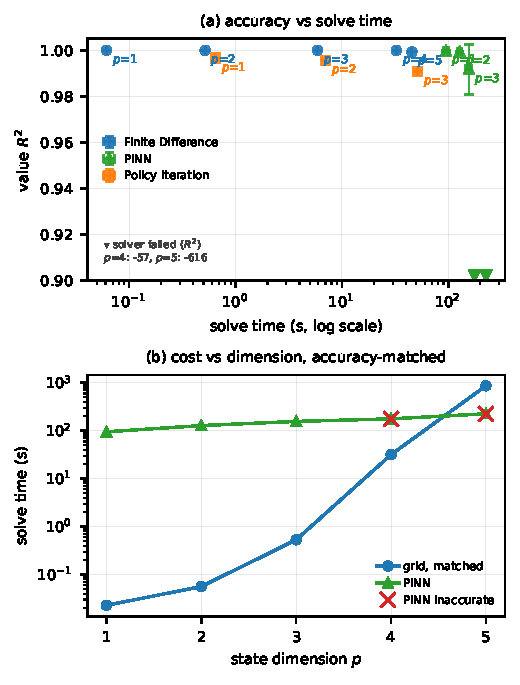
\includegraphics[width=\columnwidth]{fig1_accuracy_and_cost.pdf}
\caption{Accuracy against solve time, both families on the machine each runs well on, with the
accuracy-matched grid configuration ($N^\star = 21$) marked. Off-scale PINN failures are clipped
and annotated rather than dropped, so a reader can see where the learned solver stops solving the
problem instead of inferring it from an absence.}
\label{fig:acc_cost}
\end{figure}

Figure~\ref{fig:acc_cost} is the same comparison as a single picture: accuracy against solve time, with the accuracy-matched grid configuration marked, so
the crossing between the two families can be read off rather than assembled from columns. The
finite-difference scheme is the most accurate method
at every dimension, with value $R^2$ between $0.99927$ and $0.99999$, and its control has the
correct sign at every sampled state. Policy iteration converges in 13 outer iterations and is
slightly less accurate ($R^2 = 0.9908$ to $0.9966$), as expected from the first-order upwind
discretisation used in its policy-evaluation step.

\emph{The cost comparison does not depend on the hardware split.} Both families were timed on the
machine they run well on --- the network on the GPU, the grid sweep on the CPU --- so we also counted
work rather than seconds. Counting $3d^2 + 3m^2 + 2dm + 4d + 2$ floating-point operations per grid
point per time step, and $(6+2d)P$ per sample for the network ($P \approx 1.3\times10^4$ parameters
for training and $2P$ per query), the grid scheme converts work into time at $0.13$ to
$0.27$\,GFLOP/s while the network reaches $26$ to $30$\,GFLOP/s: a ratio of about $10^2$. Counting
work instead of seconds therefore \emph{flatters the neural solver}, which means the wall-clock
result below is the conservative one and is not an artefact of giving the network a GPU. One caveat
ran the other way in an earlier draft and is now measured rather than conceded: the grid figures come
from a NumPy implementation whose per-step cost is many small array operations, and
Table~\ref{tab:compiled} runs the same scheme as a fused parallel kernel at identical work. It is
$2.5$ to $11.9$ times faster, its achieved rate rises from $0.65$ to $7.7$\,GFLOP/s, and the two
implementations agree on the solved field to $1.3\times10^{-4}$ relative. Everything below therefore
reports both: the NumPy seconds, which are what the paper's other tables carry and which no
well-implemented grid solver would take, and what the same scheme costs compiled.

We had to reduce the grid resolution as $p$ grew, so comparing cost at the resolutions the sweep
could afford would be unfair. A separate refinement study swept $N$ at each $p$ and found the
smallest resolution reaching a fixed accuracy target of $R^2 \ge 0.9999$. That resolution is
$N^\star = 21$ at \emph{every} dimension tested, which gives one accuracy-matched grid
configuration per $p$; the grid columns of Table~\ref{tab:main} use it. Grid work grows far faster
than the point count $N^d$ suggests. The explicit time step is CFL-limited by the mesh spacing, so work
scales closer to $N^{p+1}$: at $p=5$, $N=21$ is $4.1\times10^6$ points over 420 steps, which is why
accuracy-matched finite differences cost nearly ten minutes of NumPy at a dimension the neural solver
covered in under four --- and why that is $59$\,s when the same scheme is compiled.

At matched accuracy the grid scheme is faster than the fixed-budget neural solver at every
dimension, by $5.6\times$ at $p=4$ as measured in NumPy and by $114\times$ with the same scheme
compiled, and by two to three orders of magnitude at $p \le 2$. The mesh-free solver's cost is indeed almost flat in $p$ ($95 \rightarrow 226$\,s, a factor of $2.4$
across five dimensions) against $0.023 \rightarrow 865$\,s for the NumPy grid scheme, so the two curves
do cross --- but at the crossing the neural solver is no longer solving the problem. Its accuracy
is competitive at low dimension ($R^2 = 0.9997 \pm 0.0002$ at $p=1$) and degrades with $p$,
failing outright at $p \ge 4$ under this budget. A negative $R^2$ means the learned value function
is worse than predicting the mean, so the method has not solved the problem rather than merely lost
accuracy. Control-sign agreement stays high even where $R^2$ is negative: the network recovers the
\emph{direction} of the optimal control while missing its level, so sign agreement alone is not
evidence that an HJB solver works. \emph{That failure is specific to this parameterisation, not to
the dimension} --- see Section~\ref{sec:highdim}.

% Auto-generated by src/make_tables.py -- do not edit by hand.
\begin{table}[t]
\centering
\caption{The grid timings, separated into the scheme and the implementation. The same solve --- same grid, same stencil, same step count, checked to agree on the solved field to $1.3\times10^{-4}$ relative (the edge closure; the interior is identical) --- is run by the NumPy solver used everywhere else in this paper and by a fused parallel kernel (numba; the environment has no JAX). The implementation factor grows with the problem, from $2.5\times$ at $p=1$ to $11.9\times$ at $p=4$, and the achieved rate rises --- $p=1$: $0.01\to0.01$, $p=2$: $0.14\to0.53$, $p=3$: $0.58\to4.41$, $p=4$: $0.65\to7.65$, $p=5$: $0.67\to6.43$ GFLOP/s --- which is what the FLOP model in the text was there to correct for: the NumPy figure was measuring per-step array overhead as much as arithmetic. The consequence for the comparison is at $p=5$, where the NumPy grid was slower than the neural solver ($865$\,s against $226$\,s) and the compiled one is faster ($59$\,s). Both columns are the time-stepping sweeps only, at the same forced step count.}
\label{tab:compiled}
\scriptsize
\setlength{\tabcolsep}{4pt}
\begin{tabular}{rrrrrr}
\toprule
$p$ & $N$ & steps & NumPy (s) & kernel (s) & factor \\
\midrule
1 & 21 & 420 & 0.02 & 0.009 & $2.5\times$ \\
2 & 21 & 420 & 0.05 & 0.015 & $3.7\times$ \\
3 & 21 & 420 & 0.58 & 0.076 & $7.7\times$ \\
4 & 21 & 420 & 18.48 & 1.558 & $11.9\times$ \\
5 & 21 & 420 & 567.10 & 59.252 & $9.6\times$ \\
\bottomrule
\end{tabular}
\end{table}


\subsection{Is the comparison an artefact of the quadratic solution?}\label{sec:nonpoly}

Every number above is measured on a value function that is a quadratic form, and a second-order
scheme reproduces a quadratic almost exactly. That is why the resolution needed to hit the accuracy
target came out at $N^\star = 21$ at \emph{every} dimension, which is a property of the solution
rather than of the solvers, and it is the first thing a referee should attack. The attack is
answerable, and the answer is in Table~\ref{tab:nonpoly}.

We keep the solvers and change the solution. Fix a value function that is not a polynomial,
\begin{equation}
V(x,t) = -\tfrac{1}{2}x^\top P(t)x + A_0 (T-t)\sin\!\big(\omega\,\mathbf{1}^\top x\big),
\end{equation}
with $P$ the Riccati solution so that $V(x,T) = -\tfrac12 x^\top Q_T x$ still holds, and add to the
running reward the source $s$ that makes it exact,
$s = -V_t + \tfrac12 x^\top Qx - (\nabla V)^\top Ax - \tfrac12(\nabla V)^\top BR^{-1}B^\top\nabla V
- \tfrac12\mathrm{tr}(\Sigma\Sigma^\top\nabla^2 V)$.
Then $V$ solves the HJB of the modified problem and the maximiser is unchanged --- $s$ does not
depend on $u$, so $u^\star = -R^{-1}B^\top\nabla V$ is still optimal --- which means \emph{the same
solver, the same stencil and the same CFL bound} apply, with one added term. That matters: a
reimplementation would have answered a question about the reimplementation. (Ours did, first time
round: it froze the boundary values instead of using the solver's one-sided stencils and went
unstable before producing a number.)

What changes is the physics of the question. The same accuracy target, relative $L^2$ value error
$\le 10^{-3}$, is now \emph{not reached at $N=61$ in any dimension}, where the quadratic benchmark
reached it at $N=21$ with room to spare ($R^2 \ge 0.9999$). The dimension-free resolution was
therefore an artefact of the quadratic solution. Three things are worth separating in the rest of
the table. The value error still converges at the scheme's order ($2.0$--$2.2$), so the grid method
is not degraded by the non-polynomial term --- it simply has more to resolve. The control error
converges at $1.04$--$1.13$, which is Proposition~\ref{sec:theory}'s prediction for a piecewise-linear
reconstruction and not an artefact of the quadratic either. And the cubic reconstruction keeps a
nine- to seventeen-fold advantage over the multilinear one \emph{on the same nodes}, so the paper's
headline result survives where a cubic reconstruction is no longer exact on the solution.

Two honest qualifications. First, the resolution requirement did not turn out to grow with dimension
in the way the objection anticipates: with $\omega = 3$ the dominant error is the CFL-tied time step,
which is dimension-independent, so the failure to reach the target is a statement about resolution
rather than about dimension. Push the non-polynomial term to $\omega = 12$ --- amplitude-matched, so
the control magnitude and the CFL bound are unchanged, and only the spatial scale moves --- and the
error at $N=61$ rises to $1.2\times10^{-2}$ at $d=1$ and $5.1\times10^{-3}$ at $d=2$, with apparent
orders of $2.8$--$3.1$ as the error crosses from the under-resolved spatial term to the temporal
one. The cubic's advantage shrinks to $1.7$--$2.7\times$ there, which is what one expects: when the
solve itself is wrong, a better reconstruction cannot rescue it. Second, the source is a device for
producing an exact non-polynomial solution, not a market friction; the economics of the modified
problem are artificial and we do not read anything into them. What the experiment settles is the
narrower and more important point: the accuracy comparison in this paper is not an artefact of the
benchmark's solution being a polynomial.

% Auto-generated by src/make_tables.py -- do not edit by hand.
\begin{table}[t]
\centering
\caption{The benchmark's dimension-free resolution is a property of its SOLUTION, not of the solvers. The quadratic rows are the paper's benchmark, whose value function is a quadratic form: a second-order scheme reproduces it almost exactly, and $N^\star = 21$ suffices for the accuracy target at every dimension. The non-polynomial rows replace it with a manufactured exact solution, $V = -\tfrac12 x^\top P(t)x + 5\times10^{-3}(T-t)\sin(3\cdot \mathbf{1}^\top x)$, made exact by a source in the running reward, and solved by \emph{the same solver} with the same stencil and CFL bound. The target ($\text{relative }L^2$ value error $\le 10^{-3}$) is then not reached by $N=61$ in any dimension. The control-error order and the cubic-vs-multilinear gain are given at the finest mesh: the order stays near one, as Proposition~1 predicts for a piecewise-linear reconstruction, and the cubic reconstruction keeps a nine- to seventeen-fold advantage on the same nodes --- so the paper's headline result does not depend on the solution being a polynomial.}
\label{tab:nonpoly}
\scriptsize
\setlength{\tabcolsep}{4pt}
\begin{tabular}{lrrr}
\toprule
 & $d=1$ & $d=2$ & $d=3$ \\
\midrule
\multicolumn{4}{l}{\emph{quadratic solution (this paper's benchmark)}} \\
\multicolumn{4}{l}{$N^\star$ for the target: 21, 21, 21} \\
\midrule
\multicolumn{4}{l}{\emph{non-polynomial solution (manufactured, same solvers)}} \\
value rel.\ $L^2$ at $N=61$ & 1.6e-03 & 2.0e-03 & 2.3e-03 \\
target $10^{-3}$ reached & no & no & no \\
value order vs $N$ & 2.16 & 2.11 & 2.03 \\
control order vs $N$ & 1.13 & 1.08 & 1.04 \\
cubic gain at $N=61$ & 9.3$\times$ & 16.6$\times$ & 15.5$\times$ \\
\midrule
\multicolumn{4}{l}{\emph{the same, with the non-polynomial term under-resolved ($\omega=12$)}} \\
value rel.\ $L^2$ at $N=61$ & 1.2e-02 & 5.1e-03 & -- \\
value order vs $N$ & 2.82 & 3.08 & -- \\
cubic gain at $N=61$ & 1.7$\times$ & 2.7$\times$ & -- \\
\bottomrule
\end{tabular}
\end{table}


\subsection{Value accuracy is not control accuracy}\label{sec:control}

An HJB is solved so that it can be \emph{acted on}, and what is acted on is
$u^\star = -R^{-1}B^\top \nabla V$ --- a \emph{derivative} of the value function. A grid scheme
obtains it in two steps: reconstruct the stored nodal values as a continuous interpolant, then
differentiate it. A network obtains it in one, by automatic differentiation, which is exact for
whatever function the network represents. We call the first step the \emph{reconstruction}, and its
\emph{order} the degree of the local polynomial piece it uses: one for a piecewise-linear
(multilinear) reconstruction, three for a cubic one. A reconstruction of order $k$ yields a
gradient converging at a rate set by $k$, and it is that rate --- not the accuracy of the solved
value function --- that governs the control error.

The two errors do not track each other. At every dimension and resolution tested the control error
exceeds the value error, and it converges at a stable order of about $1.00$: least-squares
fits of $\log(\text{error})$ against $\log h$ give $1.00$, $0.98$, $0.98$, $0.98$ and $0.98$ at
$p = 1,\dots,5$, with fit $R^2$ between $0.998$ and $1.000$. (Every error in this paper is a
relative $L^2$ norm, $\|a-a^\star\|_2/\|a^\star\|_2$, and every order is fitted to that error rather
than to its square --- a convention this paper previously left implicit, which is how the same
control error could be read as order $2$ in one table and order $1$ in another.) The value error
converges faster and irregularly --- $1.27$, $2.19$, $1.22$, $1.68$ and $1.85$ over the same five
dimensions --- and at the finest grid in two of the five dimensions it regresses, so the ratio
between the two grows under refinement: at $p=2$ it runs
$1.5 \to 2.2 \to 3.6 \to 5.0 \to 7.0 \to 9.1 \to 13.4$ over $N = 11,\dots,61$. The order is unchanged
by the
signal extension of Section~\ref{sec:alpha}: $1.06$ (fit $R^2 = 0.999$, over $N = 11,\dots,41$)
against $1.05$ for the inventory-only benchmark at the same state dimension, so what follows is a
property of the differentiation operator and not of the inventory-only model.

\emph{The cause is the reconstruction, not the solution.} We put the closed-form value function on
the grid as exact nodal values, so the discrete solution is error-free by construction and every
remaining control error belongs to the step that turns nodal values into a gradient. With the
multilinear interpolation and probing difference used above, that step alone reproduces almost all
of it: $6.1\times10^{-2}$ against $6.2\times10^{-2}$ at $N=11$, falling to $1.0\times10^{-2}$ at
$N=61$ at order $0.99$, against $6.2\times10^{-2} \to 1.1\times10^{-2}$ measured on the solved
grid. The grid solution is not what limits control accuracy.

\emph{What limits it is the order of the reconstruction.} Table~\ref{tab:extract} measures the
gradient-error convergence rate on functions whose gradients are known exactly, so the rates are
properties of the reconstruction rather than of this benchmark. The multilinear reconstruction is
first order on every function tested, and taking instead the \emph{exact} gradient of that same
interpolant --- the best a piecewise-linear reconstruction can do --- is also first order, so
consistency with the interpolant buys nothing. A cubic reconstruction, being $C^2$, has a smooth
rather than piecewise-constant gradient; with the table's probing step it converges at $2.2$ to
$2.8$ on the non-polynomial test functions, and with a probing step far below the mesh --- the last
two rows, which measure the reconstruction rather than the probe --- the same cubic reaches $3.4$
to $3.8$. The gap between those two numbers is worth stating plainly: a finite-difference probe
whose step is not scaled with the mesh silently caps the order a high-order reconstruction can
deliver, so the practical recommendation is not only to raise the order but to differentiate
consistently with it. Because this benchmark's value
function \emph{is} quadratic and a cubic reconstruction reproduces quadratics exactly, the last
column applies the same comparison to the Merton problem, whose closed form is a power function and
whose HJB is non-linear in the derivatives; there the cubic order is $2.6$ against $1.0$. The result
is therefore not an artefact of the linear--quadratic structure.

% Auto-generated by src/make_tables.py -- do not edit by hand.
\begin{table}[t]
\centering
\caption{The order of the reconstruction governs control accuracy, not the accuracy of the solution. Each row turns nodal values into a gradient a different way: a piecewise-linear (order-one) reconstruction whose gradient is probed by finite differences, that same reconstruction differentiated exactly, and a cubic (order-three) reconstruction probed exactly as the first. The columns report the convergence rate of the \emph{gradient} --- the control --- measured on functions whose gradients are known exactly, so the rates are properties of the reconstruction rather than of the benchmark; the first four columns are this paper's own problem, averaged over $p = 2, 3$ and $5$. Orders agreed across dimensions to within 2.0. The last column is the Merton value function, a power function from a genuinely non-linear control problem --- non-polynomial, so the cubic reconstruction is not exact there. Differentiating the piecewise-linear reconstruction exactly is no better than probing it, so consistency with the interpolant buys nothing. The quadratic column is this paper's own case and flatters the cubic method, which reproduces quadratics exactly; every other column is the one to quote. Errors are normalised by the spread of the true gradient.}
\label{tab:extract}
\small
\begin{tabular}{lrrrrr}
\toprule
 & \multicolumn{5}{c}{gradient-error convergence rate} \\
\cmidrule(lr){2-6}
reconstruction & quad. & quartic & exp. & trig. & Merton \\
\midrule
multilinear $+$ probe & 2.2 & 2.3 & 2.2 & 2.2 & 2.1 \\
multilinear, slope & 2.0 & 2.0 & 2.0 & 2.0 & 1.9 \\
cubic $+$ probe & exact & 4.8 & 4.4 & 5.6 & 5.2 \\
\bottomrule
\end{tabular}
\end{table}


\begin{figure}[!t]
\centering
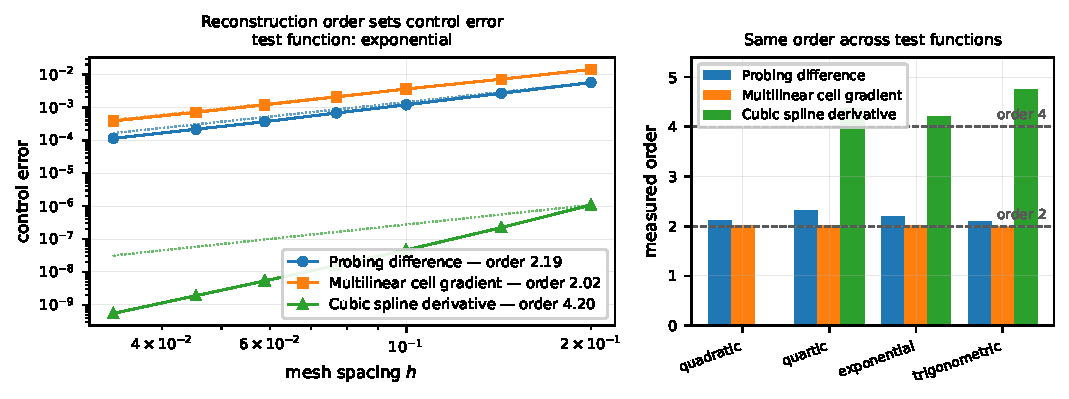
\includegraphics[width=\columnwidth]{fig_j1_control_order.pdf}
\caption{Control error against mesh spacing, on the relative $L^2$ scale used throughout. Left, the
three reconstructions on one non-polynomial test function, with a slope-$1$ reference (dotted); the
measured orders are fitted to the same data the curves show. Right, the same measurement across four
test functions, so the order can be seen to be a property of the reconstruction rather than of the
example. The cubic reconstruction is second order with the probing step used here --- third order
when that step is scaled with the mesh, as the last two rows of Table~\ref{tab:extract} show; the
quadratic case is omitted for it because a cubic spline reproduces quadratics exactly, leaving only
rounding error to fit.}
\label{fig:ctrl_order}
\end{figure}

This is why value and control accuracy can be chosen almost independently. Figure~\ref{fig:ctrl_order}
is that sentence as a measurement: control error against mesh spacing for the three reconstructions,
on the relative $L^2$ scale used throughout, with the order visible as a slope and the cubic's ceiling
visible as the point where the curve stops improving. On the benchmark's own
solved grid at $p=2$, $N=61$, the multilinear extraction gives a control error of
$1.06\times10^{-2}$ against a value error of $7.8\times10^{-4}$, a ratio of $13.6$. The cubic
extraction gives $1.3\times10^{-3}$ on the same grid, $8.2$ times smaller. There the control
error is set by the solver rather than the reconstruction, so the ratio falls to $1.7$. The
decoupling is largely an artefact of the gradient operator chosen, not a property of grid methods.

\emph{The order is a property of the reconstruction, and two points are not enough to show it.} The
comparison above rests on multilinear against cubic, and two reconstructions can be ordered by
accident. Table~\ref{tab:order} generalises it: the same nodal values are reconstructed at four
polynomial degrees, on three test functions, on a \emph{jittered} mesh, and -- the part that makes the
comparison mean anything -- every degree is differentiated by an identical rule, central differences
on its own interpolant, so nothing but the reconstruction varies across a row. The measured gradient
convergence rate rises monotonically with the degree, from $1.03$--$1.10$ at degree one to
$3.29$--$3.53$ at degree three and $5.08$--$6.34$ at degree five, and at a fixed mesh the error falls
by four to five orders of magnitude. These are the reconstruction's own rates: the probe step here
is four orders of magnitude below the mesh, which is what makes them comparable with each other. The
claim therefore holds along the whole sequence rather than
between two chosen representatives, which is what makes the recommendation actionable: a practitioner
who wants control accuracy does not choose a better solver family, they raise the order of the
operator that turns their stored values into a gradient.

% Auto-generated by src/make_order_table.py -- do not edit by hand.
\begin{table}[t]
\centering
\caption{The gradient-error convergence rate against the reconstruction's polynomial degree, on a jittered mesh. Each cell is a separate reconstruction of the same nodal values, and every degree is differentiated by the SAME rule -- central differences on its own interpolant -- so the only thing varying across a row is the reconstruction. The rate rises with the degree and the error at fixed mesh falls by four to five orders of magnitude, which makes the paper's recommendation actionable beyond the two reconstructions it was originally tested on.}
\label{tab:order}
\small
\begin{tabular}{r rrr}
\toprule
degree & exp. & trig. & rational \\
\midrule
1 & 1.05 & 1.03 & 1.10 \\
3 & 3.38 & 3.53 & 3.29 \\
5 & 5.08 & 6.00 & 6.34 \\
\bottomrule
\end{tabular}
\end{table}


One caution belongs with the degree-five row. On the exponential it first measured $2.89$ rather than
the $5$--$6$ the other functions give, and the reason is not the reconstruction: at that degree the
error reaches the floating-point floor around $10^{-10}$ and plateaus, so the last few mesh sizes
measure rounding rather than convergence and a fit across them reports an order that is far too low.
The reported figure excludes the plateau. The same trap produced a spurious order of $-2.1$ in the
earlier comparison, where a cubic reconstruction is exact on a quadratic and leaves nothing but
rounding to fit.

\emph{Refining in time cannot substitute for any of this.} Holding the mesh fixed and varying only
the number of stored snapshots separates the two errors cleanly. The value error falls by up to two
orders of magnitude ($\times4.8$, $\times12.8$, $\times20.7$ at $p=2$ for $N=21,35,45$;
$\times67.5$, $\times131.4$, $\times65.2$ at $p=3$), while the control error falls by only
$\times2.0$, $\times3.2$ and $\times4.1$ at $p=2$ and then stops improving; at $p=5$ it does not
improve at all. The plateau is not arbitrary: at $p=2$ it scales as $h$ to within measurement
error.

The resolution an application needs is therefore fixed by the control target \emph{and} the order of
the operator used to differentiate the solution --- and the second of those is free at the grid
level. That is not an argument that control error is harmless: the envelope theorem makes a control
error $\delta u$ perturb the value only by $O(\|\delta u\|^2)$, while the inventory path is a time
integral of the control and inherits its error to \emph{first} order. A solver can therefore be
accurate enough for valuation and still execute the wrong inventory.

\emph{Measured on the executed path, that is what happens.} The argument above is an argument; it can
be turned into a measurement by closing the loop. Integrating $dx = (Ax + Bu)\,dt$ from a liquidation
start under the control each reconstruction actually produces, and comparing against the exact
closed loop, separates the consequences cleanly at $N=11$ (signalled benchmark): the multilinear
extraction gives a maximum position error of $1.6\times10^{-2}$ of the initial position and an
objective loss of $1.35\%$ of $|J^\star|$, while the cubic extraction on the same nodes gives
$4.2\times10^{-3}$ and $3.9\times10^{-4}$. The ratio between the two quantities grows with refinement
--- $10.7$, $31.3$, $55.9$, $68.4$ over $N = 11,\dots,31$ --- and the fitted orders are $1.7$--$2.0$
for the position error and $2.1$ for the objective loss. Proposition~\ref{sec:theory} accounts for
both: \eqref{eq:loss} makes the loss the integral of the squared control deviation, hence second
order in a first-order control error, which is what the $2.1$ measures; and the position error is
bounded by, not equal to, the first-order inheritance $\|x_t - x_t^\star\| \le T\|B\|\sup_t\|\delta
u\|$, so an exponent above one is inside the bound rather than in conflict with it. In other words an
improvement that a value benchmark
cannot see, a $35\times$ reduction in the objective loss, is accompanied by a $4\times$ improvement
in the position actually held, and it is the position that a risk limit or an inventory constraint
acts on. One limit is worth stating: the controller is stored as snapshots and blended in time, so
its time sampling contributes about $10^{-3}$ to the position error --- comparable to the
finest-mesh figures --- and the fine-mesh rows of that comparison are therefore time-limited rather
than reconstruction-limited.

\emph{Where the error lives.} Accuracy is scored on points drawn uniformly from the state box, and a
point within one cell of the box's edge lies where the solver's stencils are one-sided and the
reconstruction has information on one side only. That band is $13\%$ of the domain at $p=1$ and
$33\%$ at $p=3$ for $N=21$ --- $41\%$ at $p=5$ by the same formula --- so a single domain-wide
average could be dominated by it without anyone noticing. It is not: the control-error density in
the band is $0.99$--$1.00$ times the interior's at $p = 1, 2, 3$, and the band contributes exactly
its share of the domain to the total squared error. Three things belong with that check. The solvers
pad the domain before building the grid, so the grid's own outermost cells are never queried at all;
the statement is about the problem domain, not the grid edge. The measurement is easy to get
backwards --- normalising the error inside each region makes the boundary look \emph{more} accurate,
because $|V|$ is largest there, which is what our first version of it reported. And one asymmetry
does survive: the cubic reconstruction's advantage is smaller in the band ($14$--$19\times$) than in
the interior ($26\times$), which is what one expects when there is no node on the far side.

\emph{What the improvement is worth in money.} The comparison above is in relative $L^2$ units, which
is not what an execution desk books. Table~\ref{tab:shortfall} closes the loop on the paper's own
real-market calibration. For each of the nine instruments the exact value function is placed on the
grid, so the solve contributes no error and the reconstruction is the only thing that differs; each
reconstruction then drives the deterministic closed loop; and the cost is the benchmark's own
objective. Its units are money once $\sigma$ and $\eta$ are relative --- $\tfrac12\int \eta u^\top u\,dt$
is the impact paid as a fraction of notional, and $10^4$ times it is basis points. Raising the reconstruction
from multilinear to cubic is worth $2.7$ to $8.4$ basis points of notional, a mean of $5.7$\,bp ---
about \$5.7k on a \$10M order --- while the cubic arm itself sits within $0.018$\,bp of the exact
control --- the pairwise difference is therefore a statement about the multilinear arm, which is what
makes it quotable. The ordering is the same one Section~\ref{sec:calib} found on the cost side and for
the same reason: the effect is largest on the \emph{most} liquid instrument, because a tighter spread
buys a larger optimal control and therefore a larger reconstruction error $\delta u \sim P\,h/\eta$.
Two measurement points belong with the number. It is the pairwise difference over the full horizon,
not the excess over the exact control truncated at $T-\delta$. Truncation removes the terminal penalty
that pays for not liquidating, so the slower arm looks cheap and the difference falls to $-0.21$\,bp at
$\delta = 0.1$. That is the same terminal contamination the paper documents for accuracy metrics, in its
cost form, with the opposite remedy: keep the horizon here, drop the terminal sample there. And the
figure is insensitive to the one coefficient that cannot be measured: across
$\lambda \in [10^{-6}, 10^{-2}]$ it moves by less than $0.002$\,bp.

% Auto-generated by src/make_tables.py -- do not edit by hand.
\begin{table}[t]
\centering
\caption{The reconstruction order in the currency it trades in. Each instrument is run through the executed closed loop with the paper's real-market calibration ($\eta$ = half the Roll effective spread, $\sigma$ from minute bars), with the exact value function placed on the grid so the solve contributes nothing and only the reconstruction differs. \emph{Excess over exact} is the cost of an arm measured against the exact control, in basis points of notional; \emph{multilinear vs cubic} is the pairwise difference, which is the well-posed statement because both arms share the snapshots and the time interpolation. The cubic arm sits at the numerical floor ($\le 0.02$\,bp), so raising the reconstruction order is worth the difference column --- and it is worth most on the MOST liquid instrument, because a tighter spread buys a larger optimal control and therefore a larger reconstruction error. Full horizon: truncating the integral at $T-\delta$ removes the terminal penalty that pays for not liquidating, which makes the slower policy look cheap (the pairwise figure falls to $-0.21$\,bp at $\delta = 0.1$ on SPY); the sensitivity is in the reproduction.}
\label{tab:shortfall}
\scriptsize
\setlength{\tabcolsep}{4pt}
\begin{tabular}{lrrr}
\toprule
instrument & $\eta$ (bp) & excess over exact: ml & ml vs cubic \\
\midrule
SPY & 1.28 & 8.42 & 8.40 \\
AMZN & 1.46 & 7.45 & 7.43 \\
MSFT & 1.58 & 6.91 & 6.89 \\
QQQ & 1.60 & 6.82 & 6.81 \\
GOOGL & 1.97 & 5.60 & 5.59 \\
OXY & 2.24 & 4.97 & 4.96 \\
NVDA & 2.68 & 4.21 & 4.20 \\
AAPL & 2.73 & 4.16 & 4.14 \\
TSLA & 4.41 & 2.69 & 2.67 \\
\midrule
\multicolumn{4}{l}{\emph{mean} 5.68\,bp of notional} \\
\bottomrule
\end{tabular}
\end{table}


\subsection{Dimension and parameterisation}\label{sec:highdim}

The sweep above stops at $p=5$ because grid methods stop being runnable past that. The analytic
reference does not: the Riccati equation is a fixed number of ODEs whatever the state dimension, so
accuracy can still be \emph{measured} where no classical baseline can be run, and we extended the
range to $p=20$. Doing so exposed a flaw in the sweep above. With the uniform defaults the value
function is \emph{separable}, $V(x,t)=\sum_i v(x_i,t)$, so solving it at $p=20$ is barely harder than
at $p=1$: the network applies one learned univariate function and sums. That is not the case the
curse-of-dimensionality argument is about.

The signal extension of Section~\ref{sec:alpha} removes the symmetry by construction rather than by
assumption: with \emph{perfectly uniform} parameters the off-diagonal block of $P$ reaches $0.205$
of the diagonal, against exactly zero here. The contrast at \emph{matched state dimension},
with the same architecture, budget and two seeds, is stark:

\begin{center}
\small
\begin{tabular}{rrr}
\toprule
$d$ & separable & with a signal \\
\midrule
2 & $+0.9994 \pm 0.0002$ & $+0.9993 \pm 0.0002$ \\
4 & $-44.5 \pm 41.2$ & $+0.9988 \pm 0.0001$ \\
6 & $-646.6 \pm 0.3$ & $+0.9968 \pm 0.0003$ \\
\bottomrule
\end{tabular}
\end{center}

\noindent At $d=4$ and $d=6$ the separable problem is not merely less accurate but unsolved --- a
negative $R^2$ means the learned value function is worse than predicting the mean --- while the
harder, genuinely multi-dimensional problem is solved to three decimals. Randomising each asset's
risk and impact coefficients reproduces the same contrast on the inventory-only problem ($-688$
against $0.981$ at $p=8$), which is how we first saw it; the signal version is the one to quote,
because it needs neither a random draw nor the claim that a particular draw is representative. The
failure is a property of the parameterisation, not of the dimension.

On the non-separable problem the PINN does not collapse; it degrades with dimension, giving
$R^2 = 0.99999$, $0.9994$, $0.9992$, $0.977$, $0.981$, $0.927$ and $0.757$ at $p = 1$, $2$, $3$,
$5$, $8$, $12$ and $20$. A grid baseline remains available and more accurate through $p=5$
(0.9999 down to 0.9993) but is not runnable at $p \ge 8$, where $N^d$ alone is $2\times10^7$ points
before the CFL-limited time step is counted. Beyond that the mesh-free solver is the only method
that runs at all --- at accuracy that declines to $0.76$ by $p=20$ and that the user cannot bound,
because nothing is left to compare against except the analytic solution we happen to have here.

The practical guidance is therefore narrower than ``PINNs fail at high dimension''. What fails is a
combination of architecture, parameterisation and budget, and the same architecture succeeds at the
same dimension once the problem is made generic --- so a PINN validated only on a symmetric toy
problem has learned nothing about either outcome.

One objection is under-training, and it deserves a direct answer. At $p=4$ the fixed budget of 6000
epochs and 2048 collocation points yields $R^2 = -44.5$ in 177\,s; 20000 epochs at the same batch
yields $R^2 = +0.9972$ in 630\,s. At $p=3$ the same increase moves $R^2$ from $0.9981$ in 172\,s to
$0.9997$ in 541\,s. Budget is therefore one lever. It is not the only one, and saying so was an
over-reach in an earlier draft of this paragraph: Section~\ref{sec:arch} shows that at the
\emph{unchanged} budget a deeper network of the same family also recovers this dimension, so the
failure is a statement about the combination in front of it, not about budget alone. What does not
change under either route is the cost: the rescued $p=4$ run took 630\,s against 31.7\,s for
accuracy-matched finite differences --- about $20\times$ more expensive, for lower accuracy
($R^2 = 0.9972$ versus $0.99991$). Since the neural solver's cost grows only slowly in $p$ while
the grid scheme's grows geometrically, the gap must close eventually, but over $p = 1$ to $5$ it
does not, and at each dimension where both methods succeed the grid scheme is faster by a factor of
$5$ to $50$ --- at the coefficients benchmarked here, a scope Section~\ref{sec:calib} measures.

\subsection{The mesh-free region is not the neural solver's alone}\label{sec:lsmc}

Everything above compares a learned solver with a mesh-based one. That leaves out the classical
family that also needs no mesh --- simulation with backward regression, the least-squares Monte Carlo
line \cite{longstaff2001valuing,glaserman2003monte} and its stochastic-control variants
\cite{kharroubi2014numerical,bender2012least} --- and leaving it out is not neutral: it is the family
a referee would name, and it decides whether the boundary drawn above is between \emph{learned} and
\emph{classical} or merely between \emph{what we ran} and \emph{what we did not}. So we run it.

The scheme is policy iteration with backward regression, on the same problem and the same reference
as the high-dimensional sweep of Section~\ref{sec:highdim}. Sample states across the domain; simulate
paths under the current policy;
regress the realised future reward at each time slice on the quadratic features
$1, x_i, x_i x_j, \tfrac12 x_i^2$; improve the policy to $u = R^{-1}B^\top\nabla V$ from the fitted
quadratic; repeat. Three implementation facts belong in the record, because each of them was needed
to make the method work at all and none of them is free. Paths must start \emph{across the domain}:
started from $x_0$ alone the cloud has radius $\sigma\sqrt{T} = 0.01$ around one corner of the box,
the fitted Hessian is meaningless, and the extracted control diverges --- to $10^{33}$ in two
iterations when we did that. The greedy update must be \emph{damped}: with a gain of $1/\eta = 100$,
a Hessian error of $10^{-3}$ is a feedback-gain error of $0.1$, and replacing the policy outright is
unstable here (we report $\alpha = 0.5$). And the regression must include the exact terminal
condition, which is part of the problem rather than part of the answer.

% Auto-generated by src/make_tables.py -- do not edit by hand.
\begin{table}[t]
\centering
\caption{Beyond the grid's limit, on the non-separable benchmark (per-asset heterogeneous risk and impact, random off-diagonal risk). The mesh-free side is not only neural: regression Monte Carlo --- a classical method that needs no grid --- runs at every dimension here, and it is more accurate than the neural solver at every dimension where both were measured, in seconds on a CPU where the neural runs take minutes on a GPU. $m$ is the number of quadratic basis functions the regression fits at every time slice, $1 + d + d(d+1)/2$: the cost of this family grows in the BASIS, not in the state dimension. That basis is also the qualification --- it is the exact structure of this benchmark's value function, which the neural solver is not given, so the result is a statement about this problem class rather than about high-dimensional HJB equations in general. PINN entries are means over its seeds at a fixed 8000-epoch budget; the grid is runnable only to $p = 5$.}
\label{tab:meshfree}
\scriptsize
\setlength{\tabcolsep}{4pt}
\begin{tabular}{rrrrrr}
\toprule
$d$ & PINN $R^2$ & RMC $R^2$ & RMC $m$ & RMC (s) & grid $R^2$ \\
\midrule
1 & $+1.0000$ & $+1.0000$ & 3 & 0 & $+0.99989$ \\
2 & $+0.9994$ & $+0.9998$ & 6 & 0 & $+0.99992$ \\
3 & $+0.9992$ & $+0.9998$ & 10 & 1 & $+0.99993$ \\
5 & $+0.9771$ & $+0.9995$ & 21 & 2 & $+0.99929$ \\
8 & $+0.9813$ & $+0.9988$ & 45 & 3 & n/a$^\dagger$ \\
12 & $+0.9269$ & $+0.9989$ & 91 & 5 & n/a$^\dagger$ \\
20 & $+0.7570$ & $+0.9771$ & 231 & 13 & n/a$^\dagger$ \\
\bottomrule
\end{tabular}
\\[2pt] {\footnotesize $^\dagger$not runnable: $N^p$ grid points at the resolution the accuracy target needs.}
\end{table}


Table~\ref{tab:meshfree} is the result, and it changes a conclusion. Regression Monte Carlo is more
accurate than the neural solver at every dimension where both were measured --- at $d=8$ by
$0.9988$ against $0.9813$, at $d=12$ by $0.9989$ against $0.9269$, and at $d=20$ by $0.9771$ against
$0.7570$ --- and it does so in $2.7$, $5.1$ and $12.5$ seconds on a CPU where the neural runs took
$196$, $270$ and $414$ seconds on a GPU. Its control is more accurate still. So ``beyond the grid's
reach the neural solver is what remains'' is false as stated; what remains is mesh-free methods, of
which one is classical, cheaper and --- here --- better.

Two qualifications keep that from being over-read, and the first is the important one. The regression
uses a quadratic basis, which is the exact structure of this benchmark's value function; the neural
solver is given no such structure. That is a real advantage and it is the reason the comparison is a
statement about \emph{this benchmark class} rather than about high-dimensional HJB equations in
general. Where the value function is not close to quadratic the basis has to be enlarged. The cost of this
family grows as $1 + d + d(d+1)/2$ basis functions (231 at $d=20$) rather than in the state dimension,
and Section~\ref{sec:nonpoly} shows what happens when the solution stops being quadratic. The honest
reading is that the classical mesh-free method wins where the practitioner
has structural knowledge, and the neural solver is the fallback where they do not.

That qualification is measured rather than asserted. Running the same regression, with the same
quadratic basis, on the manufactured family of Section~\ref{sec:nonpoly} --- whose value function is
progressively less quadratic --- gives a realised accuracy of $R^2 = 0.9998$ with the basis exactly
right ($A_0 = 0$), $0.9995$ at $A_0 = 10^{-4}$, $0.956$ at $A_0 = 10^{-3}$, and $-1.19$ to $-1.20$ at
$A_0 = 5\times10^{-3}$, which is the amplitude of the non-polynomial term used in
Section~\ref{sec:nonpoly}. At $A_0 = 2\times10^{-2}$ the run diverges: the fitted policy
drives the state out of the region the basis can describe, and the regression becomes ill-posed. The
figure at the failing amplitude is quoted as a range on purpose: within one run the seeded repeats
agree to $0.01$, but across independent runs of the same script it moves by up to $0.07$, which is
part of the finding rather than an inconvenience --- a method in a failing regime does not fail
reproducibly. So
the classical advantage is worth exactly what structural knowledge of the value function is worth, and
it fails outright --- not merely degrades --- when that knowledge is wrong by an amount this benchmark
can produce. The practitioner's decision is therefore not "classical or neural" but whether the
structural assumption can be checked, and the same repository runs the check. Second, the neural
numbers here come from a fixed 8000-epoch budget applied at every dimension rather than tuned per
dimension, and this paper's own ablation shows that budget moves the boundary; the comparison is
therefore at stated budgets, not at matched accuracy. Both point the same way for a practitioner:
the neural solver's niche is narrower than the framing it is usually given, and the measurement that
decides it is cheap to run.

\subsection{How much does the architecture choice matter?}\label{sec:arch}

Table~\ref{tab:arch} answers the objection this paper would otherwise have to concede, that a single
architecture cannot separate a property of the solver family from an artefact of the network. The
sweep is run at $p=4$, the dimension where the fixed budget collapses, because that is where an
architecture effect has room to show; a dimension where the solver already succeeds would measure
nothing. Each row is a full solve, and the grid scheme is included only for scale.

% Auto-generated by src/make_arch_table.py -- do not edit by hand.
\begin{table}[t]
\centering
\caption{Architecture sensitivity at $p=4$, the dimension where the fixed budget collapses. Every row is a full solve scored against the analytic reference; the first row is the accuracy-matched grid scheme at the same dimension, for scale. Two separate questions are answered here. Does more capacity help at a fixed budget -- yes, decisively: at 6,000 epochs the paper's $4\times64$ scores $R^2=-3.28$ while an $8\times64$ MLP, using $2.3\times$ the parameters, scores $+0.9953$. And is capacity the only lever -- no: raising the budget of the ORIGINAL architecture to 20,000 epochs reaches $+0.9972$ for less wall time than the largest network here. Both routes succeed, and both remain slower and less accurate than the grid scheme.}
\label{tab:arch}
\small
\setlength{\tabcolsep}{3pt}
\begin{tabular}{l r r r r r}
\toprule
net & ep. & params & time & value & control \\
 & & & (s) & $R^2$ & $R^2$ \\
\midrule
grid ($N=21$) & --- & --- & 20 & $+0.99991$ & $+0.99603$ \\
\midrule
2x64 shallow & 6k & 4,609 & 61 & $-337.02583$ & $-1.0963$ \\
4x64 (paper) & 6k & 12,929 & 85 & $-3.27683$ & $+0.7316$ \\
8x64 deep & 6k & 29,569 & 128 & $+0.99530$ & $+0.9969$ \\
4x128 wide & 6k & 50,433 & 79 & $+0.93647$ & $+0.9869$ \\
6x256 both & 6k & 330,753 & 100 & $+0.99672$ & $+0.9977$ \\
\midrule
2x64 shallow & 20k & 4,609 & 208 & $+0.98600$ & $+0.9874$ \\
4x64 (paper) & 20k & 12,929 & 290 & $+0.99719$ & $+0.9976$ \\
8x64 deep & 20k & 29,569 & 450 & $+0.99956$ & $+0.9993$ \\
4x128 wide & 20k & 50,433 & 288 & $+0.99974$ & $+0.9992$ \\
6x256 both & 20k & 330,753 & 351 & $+0.99757$ & $+0.9976$ \\
\bottomrule
\end{tabular}
\end{table}


Three things follow, and the third is the one that matters.

\textbf{Capacity does move the boundary.} At the paper's own 6000-epoch budget the $4\times64$ MLP
scores $R^2 = -3.28$ while an $8\times64$ MLP scores $+0.9953$ for $2.3\times$ the parameters and
$1.5\times$ the wall time. A collapse at a fixed budget is therefore not evidence that the family is
capacity-limited at that dimension; it is evidence that this architecture is.

\textbf{Depth is the lever, not width.} At the same budget the $8\times64$ network
($29{,}569$ parameters) reaches $+0.9953$ while the wider $4\times128$ ($50{,}433$ parameters)
reaches only $+0.9365$. More parameters bought a worse result, so the useful move is deeper
composition of the scaled inputs rather than a bigger final layer.

\textbf{Both routes work, and neither reaches the grid.} Raising the budget of the \emph{original}
architecture to 20000 epochs reaches $+0.9972$ in 290\,s. The 331k-parameter network is more accurate
at $+0.9976$ but costs 351\,s to get there, so on accuracy per second the small network given more
steps is the better trade --- which is the direction a practitioner should take from this table.
At 20000 epochs four of the five architectures exceed $+0.9995$ and the architecture effect is small:
what looked like a capacity story at 6000 epochs is largely a budget story, exposed by giving
capacity somewhere to go. Across all eleven configurations the best neural result is $+0.99974$ in
288\,s, against the accuracy-matched grid at $+0.99991$ in 20\,s. The separation this paper reports
therefore does not depend on which network is chosen, which is the claim the single-architecture
design could not previously support.

The sweep is over MLPs at a fixed optimiser and a fixed collocation scheme. It does not exclude
operator architectures, spectral features or curriculum on the sampling, and the honest reading of
``no architecture search'' is that this bounds the effect of capacity within one family rather than
the effect of architecture as such.


% Auto-generated by src/make_bsde_table.py -- do not edit by hand.
\begin{table}[t]
\centering
\caption{Deep BSDE, the standard high-dimensional method in mathematical finance, on the same problem and at the same dimensions as Table~\ref{tab:main}. Two columns are deliberately NOT comparable with that table and are labelled so. First, the error is measured at the single initial state the solver answers for ($x_0$, one unit of each asset), whereas the grid and PINN columns of Table~\ref{tab:main} are domain-wide: a point-valued solver is not being credited with a function-valued one's accuracy. Second, the value is quoted \emph{at its best point during training}, not at the end. In every run the terminal residual kept falling while the value error bottomed out and then degraded, so the endpoint is a factor of $14$ to $686$ worse than the number here, and a reader who trains to a residual plateau will not reproduce this column. Time is training wall time to that stopping point, at the per-epoch rate measured for each dimension in a single controlled run; that rate is nearly flat in $p$ ($0.11$--$0.15$~s per epoch), so the cost is carried by the number of epochs needed to converge, not by the cost of an epoch. One training run answers one initial state; it does not return $V$ over the domain.}
\label{tab:bsde}
\small
\setlength{\tabcolsep}{4pt}
\begin{tabular}{r r r r r r}
\toprule
$p$ & $n_{\mathrm{steps}}$ & train (s) & rel.\ err & domain var & resid. \\
 & & & at $x_0$ & & at stop \\
\midrule
1 & 200 & 309 & 0.053 & 4.22e-06 & 1.76e-03 \\
4 & 50 & 192 & 0.033 & 1.62e-05 & 5.21e+00 \\
8 & 50 & 759 & 0.003 & 2.76e-05 & 7.17e-01 \\
\bottomrule
\end{tabular}
\end{table}


\begin{figure}[!t]
\centering
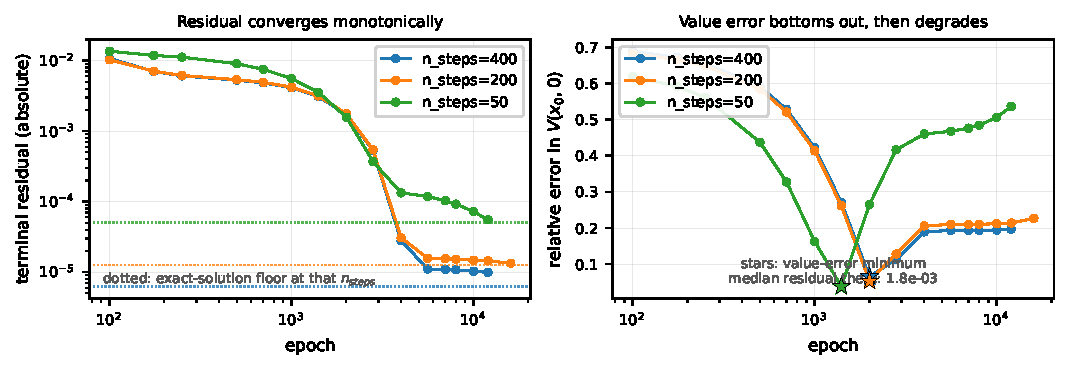
\includegraphics[width=\columnwidth]{fig_j2_bsde_stopping.pdf}
\caption{Deep BSDE: the terminal residual converges, the value does not. Left, the residual falls
monotonically at every resolution, approaching the discretisation floor of the scheme it is solving
(dotted). Right, the same runs' relative error in $V(x_0,0)$ bottoms out and then \emph{grows}
(stars mark each minimum). Training to a residual plateau therefore overshoots the best value the
run passes through, by a factor of $14$ to $686$ depending on dimension --- which is why
Table~\ref{tab:bsde} quotes the value at its minimum and not at the end.}
\label{fig:bsde_stop}
\end{figure}

The omission that most needs answering is deep BSDE, which is the standard high-dimensional method in
mathematical finance and which we therefore ran rather than merely cited. Table~\ref{tab:bsde} gives
it on the same problem at $p=1$, $4$ and $8$, and the comparison is deliberately narrow: deep BSDE is
point-valued, so its error is measured at the single initial state it answers for, not over the
domain as the grid and PINN columns of Table~\ref{tab:main} are. Two things follow.

First, where the grid scheme can run, deep BSDE does not reach its accuracy. At $p=1$ and $p=4$ its
best value error is $5.3\%$ and $3.3\%$, against value $R^2$ of $0.99995$ and $0.99992$ for
accuracy-matched finite differences, and its terminal residual at that point is still $71\times$ and
$2.6\times 10^4\times$ the discretisation floor of the scheme it is solving. So the conclusion of
Table~\ref{tab:main} is not an artefact of having chosen the PINN as the neural representative: the
other standard neural family, measured rather than assumed, loses to the classical scheme on the same
axis in the regime where the classical scheme is available.

Second, and in the other direction, deep BSDE is the strongest of the learned solvers where the grid
is not runnable. At $p=8$ it reaches $0.35\%$ relative error on $V(x_0,0)$, while the PINN reaches
$R^2 = 0.977$ and the grid scheme is $2\times10^7$ points before its CFL-limited time step is counted.
The cost is not the per-epoch rate --- that is nearly flat in $p$, $0.11$ to $0.15$\,s --- but the
number of epochs needed to reach the stopping point, which rises from $2000$ at $p=4$ to $6000$ at
$p=8$.

One caution belongs with any deep-BSDE number, and Figure~\ref{fig:bsde_stop} is the reason. In every
run the residual kept falling while the value error degraded, reaching $1268\%$ by the end of the
$p=4$ run. The stopping point is consequently part of the reported configuration. It does not
transfer between dimensions: the absolute residual threshold that is optimal at $p=1$ is three orders
of magnitude too late at $p=4$. A scale-free version still moves by a factor of $31$ across the
dimensions we measured, so the stopping point has to be found by monitoring the value rather than by
a rule.

\emph{And the family's modern member.} A referee is entitled to answer the above with ``then compare
against a strong variant''. Deep splitting \cite{beck2019deep} is that variant: instead of one
time-global network it fits one small network per time step by regression on simulated paths, and we
implement it, validate it and run it on the same benchmark. The scheme itself is sound here --- running
the same recursion with the per-step regression solved exactly in the quadratic basis, which is the
solution's own functional form, gives value $R^2$ of $0.9987$, $0.9960$ and $0.9939$ at $d = 1, 4, 8$
--- but the neural realisation does not reach it: $0.16$, $-76$ and $-286$ at the same step count, with
the median per-step regression loss degrading from $0.05$ to $1.0$ over the same range. The
discrepancy is therefore the learner's, not the scheme's, and the mechanism is the one this paper is
about. The recursion feeds the \emph{gradient} forward: $z = \Sigma^\top\nabla u$ enters
$f = -\tfrac12 x^\top Qx + \tfrac12 z^\top M z$ with $M = \Sigma^{-1}BR^{-1}B^\top\Sigma^{-\top}$
of order $10^6$, so a per-step regression is asked for gradient accuracy, while a mean-squared-error
loss constrains the function and not its derivative. This is the value/control decoupling of
Section~\ref{sec:control} reappearing inside a neural solver, with the same practical reading: a
splitting implementation validated on its value residual can be worthless in the value it reports
while its control looks reasonable --- $R^2$ of $0.86$ on the control against $0.16$ on the value at
$d=1$. Deep splitting is not a weak method; on this benchmark it is a method whose per-step regression
has to be accurate in a derivative, and we report both arms so that the reader can see which one the
limitation belongs to.

That the limitation is neither the training budget nor the network's capacity is measured rather than
assumed. At a fixed 50 steps, moving from $2\times32$ and 300 epochs per step to $4\times64$ and 2000
--- $6.7\times$ the gradient steps --- improves the median per-step fit by $179\times$ (to
$2.7\times10^{-4}$), and moves the value $R^2$ from $+0.16$ to $-16.5$: a better fit to each step's
target produces a worse value function, while the control $R^2$ stays between $0.86$ and $0.89$
throughout. The corresponding check on the mechanism is direct: at the trained networks the
\emph{relative} error of the recovered gradient exceeds that of the value by $1.6$ to $4.3\times$ at
the steps we measured (with one exception near $t=0$), which is what a loss constraining the function
rather than its derivative predicts, and it is the gradient that the recursion feeds forward.

\subsection{The classical probabilistic method, where it applies}\label{sec:mlp}

The last family to place is the one with a complexity theory behind it, and
Table~\ref{tab:mlp} gives both what it achieves and the condition under which it achieves it.
Multilevel Picard
\cite{hutzenthaler2020multilevel,hutzenthaler2022overcoming} approximates a high-dimensional semilinear PDE at a point by
realising the Picard iteration in a full-history multilevel Monte Carlo scheme, and it is the classical
method the deep-learning literature is usually measured against on high-dimensional problems. We
implement it in the published form, with one deviation stated rather than hidden: our nonlinearity
consumes the \emph{gradient}, so $\nabla U_\ell$ is obtained by central differences with step
$\varepsilon$ --- the practical route for gradient-dependent nonlinearities
\cite{neufeld2023multilevel} --- rather than by the Beta-time-sampled variant that reference
introduces for exactly this case. Two consequences follow, and the second is the finding.

% Auto-generated by src/make_tables.py -- do not edit by hand.
\begin{table}[t]
\centering
\caption{Multilevel Picard, measured rather than cited. \emph{Upper}: the method realises the Picard iteration, so it needs that iteration to be a contraction, with Lipschitz constant $|\nabla V|/\eta$. Sweeping $\eta$ from weak control authority to strong locates the boundary between $|\nabla V|/\eta = 0.56$ (converged) and $0.91$ (diverged) instead of leaving it as a caveat. \emph{Lower}: the same HJB family at $d = 1$ to $20$. At the paper's own calibration the scheme diverges at every dimension --- in a tenth of a second, so this is the hypothesis failing rather than a budget running out --- while at $\eta = 1$ it is the cheapest method in this paper, $0.26$\% at $d=20$ in $2.3$\,s on a CPU, where no grid can run and where the PINN reaches $R^2 = 0.757$. The implementation is checked where the hypothesis holds: at $\eta=1$ the relative error falls $6.7e-03 \to 1.5e-03$ from level 2 to level 4.}
\label{tab:mlp}
\footnotesize
\setlength{\tabcolsep}{4pt}
\begin{tabular}{rrrr}
\toprule
\multicolumn{4}{l}{\emph{contraction boundary at $d=1$}} \\
$\eta$ & $|\nabla V|/\eta$ & level-3 rel.\ err & verdict \\
\midrule
$10$ & $0.011$ & $7.02e-03$ & converged \\
$1$ & $0.100$ & $6.37e-03$ & converged \\
$0.3$ & $0.275$ & $1.06e-02$ & converged \\
$0.1$ & $0.557$ & $2.12e-02$ & converged \\
$0.03$ & $0.907$ & $4.38e+00$ & diverged \\
$0.01$ & $1.249$ & $8.21e+02$ & diverged \\
\midrule
\multicolumn{4}{l}{\emph{across dimension, $M=2$, 3 levels}} \\
$d$ & rel.\ err at $\eta=0.01$ & rel.\ err at $\eta=1$ & time at $\eta=1$ (s) \\
\midrule
$1$ & $82115$\% & $0.637$\% & $0.00$ \\
$4$ & $582833$\% & $0.439$\% & $0.05$ \\
$8$ & $551822$\% & $0.425$\% & $0.20$ \\
$12$ & $433216$\% & $0.173$\% & $0.58$ \\
$20$ & $201008$\% & $0.258$\% & $2.25$ \\
\bottomrule
\end{tabular}
\end{table}


First, where the method's hypothesis holds it is the strongest thing in this paper, and not narrowly.
MLP realises the Picard iteration, whose Lipschitz constant here is $|\nabla V|/\eta$; at $\eta = 1$
(a wider spread, i.e.\ weaker control authority) that is $0.10$ and the iteration converges. It then
reaches $0.26\%$ relative error on $V(x_0,0)$ at $d = 20$ in $2.3$ seconds on a CPU, against
$R^2 = 0.757$ for the PINN on the same problem, $0.977$ for regression Monte Carlo (in $12.5$\,s, and
with a hand-chosen basis), and no grid at all. The implementation is checked where the hypothesis
holds --- the relative error falls $6.7\times10^{-3}$ to $1.5\times10^{-3}$ from level 2 to level 4 ---
so the divergence below is the method's condition and not a defect in our code.

Second, at the paper's own calibration it does not converge, and the boundary is measurable rather than
mysterious. The Picard map's Lipschitz constant at $\eta = 0.01$ is $1.25$: above one, so the iteration
is not a contraction and the iterates diverge. Sweeping $\eta$ locates the transition between
$|\nabla V|/\eta = 0.56$ (converged) and $0.91$ (diverged). The divergence is not a budget running out
--- the $d=20$ run that diverges takes $1.8$\,s --- and it is not the finite-difference gradient, whose
step we varied over two orders of magnitude with no effect on the outcome. It is the same stiffness
that sets the grid's CFL limit and destabilises the explicit splitting recursion: the maximised
Hamiltonian $\tfrac12\nabla V^\top BR^{-1}B^\top\nabla V$, whose coefficient is $1/\eta$, is what has
to be handled carefully by anything that touches it, and multilevel Picard touches it through a
contraction. This is the third method in this paper to be limited by that one term, and it is the term
the optimal-execution literature treats as a modelling constant rather than as a numerical parameter.

\subsection{Market-calibrated scope}\label{sec:calib}

% Auto-generated by src/make_calibration_table.py -- do not edit by hand.
\begin{table}[t]
\centering
\caption{The explicit grid scheme's time-step requirement under measured liquidity. $\eta$ is half the Roll effective spread \cite{roll1984simple} measured on the causal minute data, with Corwin--Schultz \cite{corwin2012simple} as a cross-check. The optimal control is $u^\star = -R^{-1}B^\top P x$ with $R = \eta I$, and the explicit time step is CFL-limited by $dt \le 0.25\,dx/\|u^\star\|_\infty$, so a smaller $\eta$ buys a larger control and a proportionally smaller step. Everything else is held at the paper's synthetic values, so the column is a statement about the instrument's liquidity alone. The ordering is the point: the most liquid instrument pays the largest penalty.}
\label{tab:calib}
\small
\begin{tabular}{l r r r r}
\toprule
 & half-Roll & $\max|u^\star|$ & time & vs.\ synthetic \\
instrument & spread $\eta$ & on grid & steps & calibration \\
\midrule
synthetic & 1.00e-02 & 12.5 & 800 & $1\times$ \\
\midrule
SPY & 1.28e-04 & 975 & 62,427 & $78\times$ \\
AMZN & 1.46e-04 & 858 & 54,889 & $69\times$ \\
MSFT & 1.58e-04 & 792 & 50,713 & $63\times$ \\
QQQ & 1.60e-04 & 781 & 50,016 & $63\times$ \\
GOOGL & 1.97e-04 & 634 & 40,547 & $51\times$ \\
OXY & 2.24e-04 & 557 & 35,667 & $45\times$ \\
NVDA & 2.69e-04 & 466 & 29,795 & $37\times$ \\
AAPL & 2.73e-04 & 458 & 29,342 & $37\times$ \\
TSLA & 4.41e-04 & 283 & 18,124 & $23\times$ \\
\bottomrule
\end{tabular}
\end{table}


Everything above uses coefficients that were chosen, not measured: $\eta = \lambda\sigma^2 = 0.01$ and
$Q_T = 0.1$. A benchmark is entitled to do that, but the entitlement expires when its conclusions are
read as statements about trading, so this subsection asks what happens when the coefficients come
from the data instead. Table~\ref{tab:calib} answers it for the impact coefficient.

Two of the three are measurable and one is not. The diffusion scale is the relative volatility, which
we take from the minute bars. The impact coefficient is not observable, and we identify it with half
the Roll effective spread \cite{roll1984simple} -- a round trip pays the spread once, so a unit trade
pays about half of it -- using the estimator already computed on the causal data and cross-checked
against Corwin--Schultz \cite{corwin2012simple}. Risk aversion is a preference. Nothing in a price
series determines it, so any single calibrated value would be a choice dressed as a measurement.

That last point sets the design rather than excusing it. On this problem the pinned quantity is
$k = \sqrt{Q/\eta} = \sigma\sqrt{\lambda}/\sqrt{\eta}$, which fixes how fast the position is
liquidated. Measured liquidity with a defensible $\lambda \in [10^{-6}, 10^{-2}]$ puts $k$ between
$0.001$ and $0.15$; our synthetic coefficients sit at $k = 1$. The benchmark therefore liquidates
roughly an order of magnitude faster than real liquidity and realistic risk aversion imply. We
sweep $\lambda$ across that range rather than picking from it, so the results below are a statement
about robustness and not about a chosen calibration.

\textbf{Accuracy is unaffected.} Across thirteen configurations -- SPY, AAPL, NVDA and TSLA, each at
three values of $\lambda$, at $p = 1$ -- the grid scheme scores value $R^2$ between $+0.99996$ and
$+0.99997$ against $+0.99999$ at the synthetic coefficients, with control $R^2$ unchanged at
$+0.9990$. The control-to-value error ratio, the quantity Section~\ref{sec:control} is built on,
lands between $7.9$ and $16.4$ across every configuration, against $16.4$ synthetic. Real
coefficients move neither the accuracy of the classical scheme nor the size of the control/value gap.

\textbf{Cost does not survive, and this is the finding.} The optimal control is
$u^\star = -R^{-1}B^\top P x$ with $R = \eta I$, so a smaller impact coefficient buys a
proportionally larger control; the explicit scheme's step is CFL-limited by
$dt \le 0.25\,dx/\|u^\star\|_\infty$; and the step count therefore scales as $1/\eta$.
Table~\ref{tab:calib} evaluates that at each instrument's own measured spread, holding everything else
at the paper's values. The tightest instrument in the collection, SPY, needs $78\times$ the synthetic
run's time steps; the widest, TSLA, needs $23\times$. The ordering is the opposite of the
intuitive one: liquidity is what makes the explicit scheme expensive here, not illiquidity.

So the paper's speed claim has a narrower scope than its accuracy claim, and we state it that way.
Where a grid scheme can run it is faster than the mesh-free solver \emph{at the coefficients
benchmarked here}; transferring that to a specific instrument requires the step count to be redone at
that instrument's spread. Two qualifications keep this from over-reading. It constrains the
\emph{explicit} scheme, which is the one our cost tables use; our implicit variant
(Section~\ref{sec:disc}) removes the stability restriction at four times the explicit step, but it was
measured at the synthetic $\eta$ only, so nothing here says an implicit scheme is slow at real
spreads. And a step count is work, not wall-clock: the grid's per-step cost is the point count, so the
ratio of step counts is the ratio of work for a fixed mesh.

One methodological consequence is worth recording because it cost us a wrong result first. The
accuracy function samples query times with \texttt{linspace}, which includes $t = T$, and the
reference control diverges there -- the last instant of a liquidation problem wants to trade
infinitely fast. At the synthetic $\eta$ the terminal sample is mild, with mean $|u^\star| = 5.1$
against $0.6$ to $1.7$ in the interior, and excluding it moves control $R^2$ by less than $10^{-4}$.
At SPY's $\eta$, smaller by $78\times$, the terminal sample reaches $395$ and a solve that is accurate
in the interior is scored at value $R^2 = -997$. The estimator is therefore not the difficulty; the
sampling is, and any evaluation at real spreads has to drop the terminal sample.

%=====================================================================
\section{Discussion and Limitations}\label{sec:disc}
%=====================================================================

\subsection{When to use which}
Table~\ref{tab:guide} states the recommendation the comparison supports. Every row is a regime a
practitioner can recognise before committing to a method, and every recommendation points at a
measurement in this paper rather than at a preference. The neural solver is preferred in only two
rows, and in both the reason is that the classical scheme cannot be run or should not be re-run ---
not that it was beaten on accuracy; where the two can be compared, the classical scheme wins on both
axes.

% The decision guide: which method to use, when, and the measurement that decides it.
%
% Hand-written rather than generated, because it is an argument rather than a dump of results:
% every row points at a measurement made elsewhere in the paper. Kept to one column; the
% "deciding measurement" column carries the number so a reader can check it against the tables.
\begin{table}[!tb]
\centering
\caption{Which solver to use. Each row is a regime a practitioner can recognise before solving
anything, and the evidence is a measurement reported in this paper rather than a preference. The
recommendation is deliberately conditional: the two rows that prefer the neural solver are cases
where the classical scheme \emph{cannot} be run or \emph{should not} be re-run, not cases where it
is beaten on accuracy.}
\label{tab:guide}
\small
\setlength{\tabcolsep}{3.2pt}
\begin{tabular}{@{}p{0.20\columnwidth}p{0.30\columnwidth}p{0.40\columnwidth}@{}}
\toprule
Regime & Use & Deciding measurement \\
\midrule
Single instance, $p \le 5$ & \textbf{grid scheme} & faster \emph{and} more accurate everywhere it
runs: factor $5$--$50$ in time at $p=4$--$5$, two to three orders at low $p$ (Table~\ref{tab:main}) \\
\addlinespace
Control accuracy matters, not just value accuracy & \textbf{grid scheme}, and raise the
reconstruction order & a cubic reconstruction on the same nodes cuts the control error
$4$--$5$ orders of magnitude and the control/value ratio from $185$ to $2.8$
(Table~\ref{tab:extract}) \\
\addlinespace
$p \ge 8$ & \textbf{neural}, the only method that runs & the grid needs $N^p$ points;
at $N=21$, $p=8$ is $2\times10^{7}$ before the CFL-limited time step is counted
(Section~\ref{sec:highdim}) \\
\addlinespace
A family of $\gtrsim 10^3$ problems & \textbf{learned operator} & the classical scheme must be
re-solved per instance; an operator amortises after $1{,}000$ to $4{,}365$ parameter settings \\
\addlinespace
Accuracy must be known, not assumed & \textbf{grid scheme} & the neural solver's accuracy decays
from $R^2 = 0.98$ at $p=8$ to $0.76$ at $p=20$ while its control-sign agreement stays near $0.7$:
no internal signal of the decay (Section~\ref{sec:highdim}) \\
\addlinespace
Inputs will leave the training domain & \textbf{scale them explicitly}, whichever solver &
an unscaled network's price sensitivity decays monotonically with price level, rank correlation
$-0.90$ to $-1.00$, so any threshold on it yields an artefact (Section~\ref{sec:ood}) \\
\bottomrule
\end{tabular}
\end{table}


\subsection{One problem or a family}
A natural objection is that the comparison should use inference time rather than training time, since
a trained network evaluates in microseconds. We measured both, and the objection does not hold here:
both methods have an expensive offline solve followed by cheap online queries. Amortised over one
trading day of minute decisions the grid scheme's interpolation costs 0.66\,$\mu$s at $p=1$ and
34.3\,$\mu$s at $p=5$, against 3.0--4.9\,$\mu$s for the PINN on GPU, so the neural solver's
inference is \emph{not} uniformly faster. Combining the terms as
$T(N) = T_{\text{offline}} + N\,t_{\text{eval}}$, the PINN never breaks even at $p=1$, and at $p=5$
it is finally cheaper on \emph{both} terms ($226$\,s against an $865$\,s solve) only where it is not
accurate ($R^2 = -616$): the binding constraint has moved from cost to accuracy.

The regime changes for a \emph{family} of problems. Where the solver must be re-solved for every
member, the break-even count with $10^3$ training solves is $4{,}365$ instances at $p=2$ and
$1{,}000$ at $p=5$ --- essentially the size of the training set, and \emph{falling} as dimension
rises --- so an \emph{operator} amortises after $1{,}000$ to $4{,}365$ parameter settings, which is
exactly the regime a calibration study occupies. A fixed-parameter PINN does not, and most operator
architectures would need labelled solutions from the solver they aim to replace, though the
physics-informed family \cite{wang2021physics} trains on the residual and needs none.

\emph{Operator learning, and why it is a different axis.} The field has moved from fixed architectures
--- the spectral convolutions of \cite{li2021fourier}, the branch/trunk construction of
\cite{lu2021learning}, and the discretisation-invariance arguments of \cite{raonic2023convolutional} ---
towards models pretrained across families of equations and specified at query time by examples rather
than by weights \cite{yang2024pde}. None of that is a solver for one instance, which is what this
paper measures, and it is worth being explicit about the consequences rather than adding a row that
would not be comparable. An operator is trained on a \emph{family}, so the honest comparison is an
amortised one: train once, evaluate on held-out members, and charge the classical methods a full
re-solve per member. That comparison is well posed here --- every member has a closed-form reference --- and we have not
run it, for a reason that is a property of this benchmark rather than a preference. The operator's
input would be a low-dimensional parameter vector $(\lambda, \sigma, \eta, x_0)$, so the exercise would
test whether a network can learn a smooth map from a handful of numbers. The methods already in this
paper solve the same problem to a fraction of a percent in seconds: regression Monte
Carlo at $0.4\%$ relative error at $d=1$, rising to $3.4\%$ at $d=20$, and multilevel Picard at
$0.26\%$ at $d=20$. Operator learning earns its place when the input is a \emph{function} --- a volatility
surface, an order-flow signal, a whole price path --- which is the signalled and market-calibrated
extension of Section~\ref{sec:alpha} rather than the benchmark itself, and that is where we would place
it.

One connection is worth stating because it is not obvious and it is a prediction. Proposition~1
is not about grid schemes: it says that any solver whose delivered object is a \emph{derivative} of a
reconstructed field inherits the reconstruction's order, and that a differentiation step caps it. An
operator that outputs the value function and whose control is then obtained by differentiating the
output --- finite differences, or autograd of a network whose smoothness is set by its architecture ---
is in exactly that position, so the recommendation of Section~\ref{sec:control} transfers: if control
accuracy matters, raise the order of the reconstruction before changing the solver. We state it as a
prediction because we did not measure an operator on this benchmark, and the benchmark is released so
that it can be tested against a closed-form reference.

\subsection{Out-of-domain evaluation}\label{sec:ood}
A surrogate trained on a normalised state domain and evaluated in physical units fails quietly. A
$4\times64$ $\tanh$ MLP trained on the HJB residual with terminal condition
$V(S,T) = -\tfrac{1}{2}(S-25)^2$ on prices sampled from $[20,30]$ only, then evaluated on the
realised price levels of the nine instruments (\$42 to \$536), shows a learned price sensitivity
$|\partial V/\partial S|$ that falls monotonically with price --- from $3.36$ at \$42 to $0.062$ at
\$536, a factor of about 54 --- with rank correlations of $-0.90$, $-0.98$ and $-1.00$ across three
seeds. The network saturates in proportion to how far its input lies beyond the training domain, so
any threshold applied to this gradient inherits the ordering and produces a cross-sectional
``finding'' that admits a plausible microstructure story while being entirely an artefact of scale.
Mapping the input back into the training domain removes the dependence ($+0.12$, $-0.22$, $+0.23$).
What we add to the known out-of-domain failure of learned operators \cite{chandra2024uncertainty}
is its \emph{shape} in a control setting --- saturation rather than divergence, so the damage
survives every sanity check that looks for obviously broken output --- and the procedural
recommendation that follows: report per-channel input coverage for every evaluation set.

\textbf{Limitations.} (i) The cost half of the argument stops at $p \approx 5$, where the grid
scheme stops being runnable at the resolution the accuracy target needs. That limit deserves one
qualification, because the obvious objection to it is the wrong one. The restriction is not the CFL
condition as such: we implemented the diffusion implicitly, by one-dimensional splitting, and it is
stable and accurate at four times the explicit step (value $R^2$ still $0.999$). But splitting is
only first-order in time, so holding the temporal error below the spatial error still requires
$dt \sim dx^2$ --- the same rate the CFL condition imposes --- and what implicitness buys is a
constant factor of about four rather than a change in the scaling. The limitation is therefore the
cost of controlling the temporal error, not stability; moving it needs a second-order time
integrator, or sparse grids \cite{bungartz2004sparse}, which attack the $N^d$ factor instead. (ii) The neural results use one
architecture ($4\times64$ $\tanh$), one optimiser and one schedule. Section~\ref{sec:arch} measures
what that choice is worth \emph{within} the family --- capacity and budget each move the boundary at
$p=4$ --- but the sweep is still over MLPs at a fixed optimiser and fixed collocation, so it bounds
the effect of size rather than of architecture as such. Techniques for high-dimensional PDEs
\cite{meng2020ppinn,moseley2021finite} could plausibly shift where the boundary sits, and so could
architectural choices deliberately left out of scope here -- wider
residual blocks \cite{zagoruyko2016wide}, or input feature maps that change the network's spectral
bias and therefore which scales it can represent \cite{wang2020understanding} -- and we release the
benchmark so that such claims can be tested against a closed-form
reference. (iii) The separability effect is established as a phenomenon, not explained: we do not
claim that symmetry \emph{causes} the failure. (iv) Timings come from a single GPU and CPU, and the
comparison is stated as GPU-for-neural versus CPU-for-grid, which favours the neural solver. (v) The
control-accuracy result assumes a solver whose control is a finite difference of an interpolated
value function; a scheme that solves for the control directly could narrow the gap, and we have not
tested it. (vi) The model coefficients are synthetic rather than calibrated to an instrument, so no
result here is a statement about how a particular asset trades. Section~\ref{sec:calib} measures what
calibration does to the conclusions, and the answer is not uniform: the \emph{accuracy} comparison is
unchanged, while the \emph{cost} comparison is not, because a market-calibrated impact coefficient
multiplies the explicit scheme's time-step requirement by $23$--$78\times$ depending on the
instrument. The speed claim therefore carries the scope stated in Section~\ref{sec:calib} and not a
general one. What the paper supplies no evidence about, under any calibration, is realised trading
performance, and we offer none.

%=====================================================================
\section{Conclusion}
%=====================================================================

We compared neural and classical solvers for the HJB equation of multi-asset optimal execution
against a closed-form Riccati reference. The comparison produces a boundary rather than a winner,
because the two families are not ranked along one axis but along three. Wherever a grid scheme can
run, up to about five state dimensions, it is both faster and more accurate --- by $5.6\times$ at
$p=4$ as measured in NumPy and $114\times$ with the same scheme compiled, which is also what flips
the one dimension where the NumPy grid had been the slower method. Where it cannot run, the classical side is still not finished: regression Monte
Carlo also needs no grid, and it beats the neural solver at every dimension where both were measured
($R^2$ of $0.999$ at $p=12$ and $0.977$ at $p=20$ against $0.927$ and $0.757$), in seconds on a CPU rather than minutes on a GPU. Multilevel Picard does better still where its
hypothesis holds --- $0.26\%$ at $p=20$ in $2.3$ seconds --- though at this paper's own calibration the
Picard iteration it realises is not a contraction and it diverges, with the boundary measured. The
neural solver's accuracy also decays with no internal signal
that it is decaying, which is the property a practitioner cannot work around.

Measuring the \emph{control}, which is what an HJB is for, says something more useful: value
accuracy does not bound control accuracy, because what limits the control is the order of the
operator that turns nodal values into a gradient. A multilinear reconstruction is first order, its
exact gradient is also first order, and a cubic reconstruction on the same nodes reaches order
$2.4$ with the same probing step and $3.4$ when that step is scaled with the mesh, cutting the
control/value error ratio from $13.6$ to $1.7$ --- worth $2.7$ to $8.4$ basis points of notional on
the paper's own market calibration, and largest on the most liquid instrument. That improvement is
free at the grid level, which is
why the actionable recommendation is
the second row of Table~\ref{tab:guide}: if control accuracy matters, change the reconstruction
before changing the solver.

Two objections changed the picture without reversing it. A larger training budget recovers accuracy
a smaller one loses, and we report the rescued run rather than the flattering comparison. And the
field's preference for inference time is justified, because a classical solver must be re-solved for
every instance --- but the two framings answer different questions, one problem or a family of them,
and have opposite answers. One term links the three limitations above: the maximised Hamiltonian
$\tfrac12\nabla V^\top BR^{-1}B^\top\nabla V$, whose coefficient is $1/\eta$, sets the grid's
time-step limit, destabilises the explicit splitting recursion, and breaks multilevel Picard's
contraction. The reconstruction question and the stiffness question are therefore the same question,
and it is asked about the one coefficient the optimal-execution literature treats as a modelling
constant. Both generalise: validate on the problem you actually have, with a reference you can trust.

\section*{Reproducibility}
Code, the temporal data splits, the preprocessing manifest and every raw result file behind the
tables are released at \repourl. The reference is checked against three
independent closed forms, and the manuscript is built and page-checked by
\texttt{src/build\_paper.py}.

\bibliographystyle{IEEEtran}
\bibliography{refs}

\end{document}
